%
% Firewall
%
% Aleph Objects Firewall
%
% Copyright (C) 2014, 2015, 2016 Aleph Objects, Inc.
%
% This document is licensed under the Creative Commons Attribution 4.0
% International Public License (CC BY-SA 4.0) by Aleph Objects, Inc.
%
\begin{figure}[h!]
\begin{center}
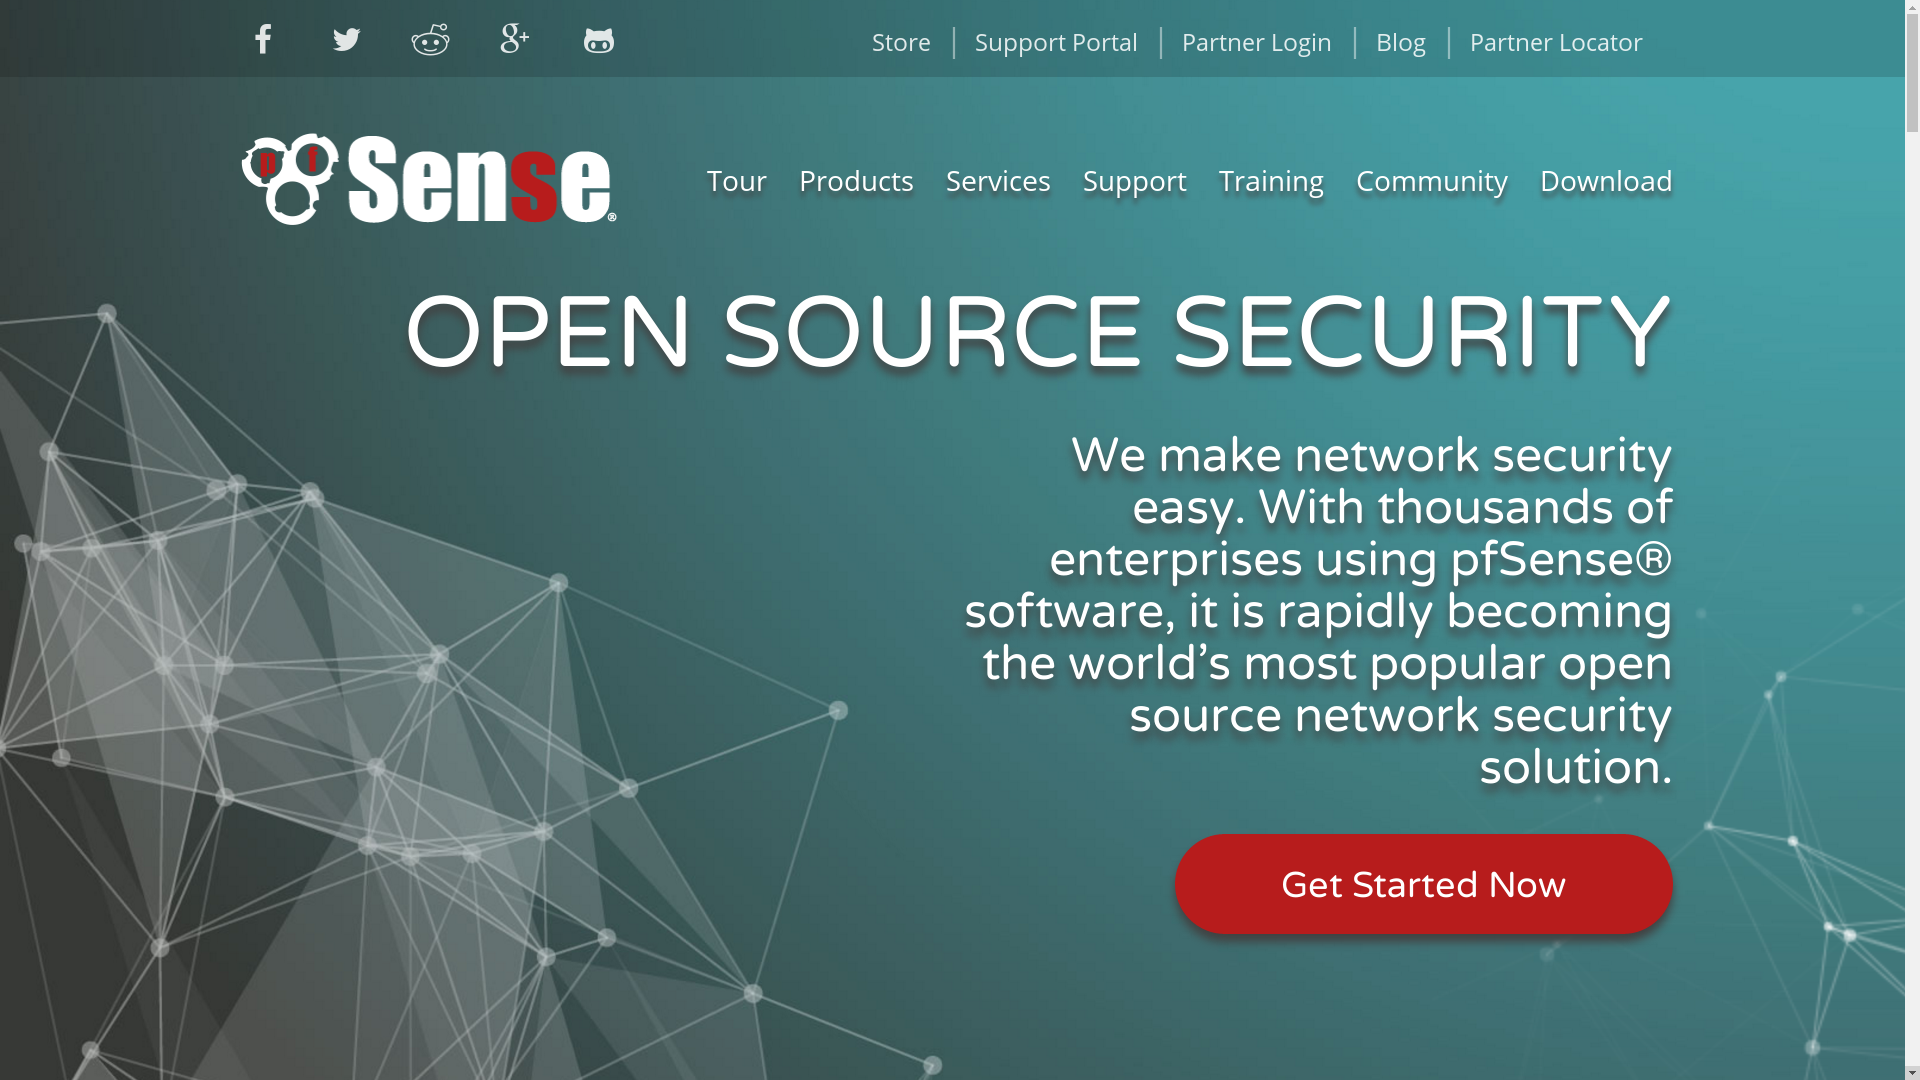
\includegraphics[keepaspectratio=true,height=1.10\textheight,width=1.00\textwidth,angle=0]{www-pfsense.png}
 \caption{pfSense Website}
 \label{fig:www-pfsense}
\end{center}
\end{figure}

\section{Overview}
Aleph Objects has recently deployed pfSense firewalls, replacing OpenBSD.

\href{https://www.pfsense.org/}{pfSense} --- ``Free, open source customized
distribution of FreeBSD specifically tailored for use as a firewall and router
that is entirely managed via web interface.''

pfSense was selected as Aleph Objects core router/firewall for backbone
connections.

\section{Initial Configuration}

These are the the initial configuration steps for a pfSense firewall. Here is an overview of the steps:

\begin{enumerate}
 \item Make serial connection to pfSense firewall, and do basic initial setup.
 \item Connect via ethernet to pfSense firewall with web browser.
 \item Do more initial setup.
 \item Connect pfSense router to Internet.
 \item Update router.
 \item Install new packages.
 \item Configure packages.
 \item Backup \& reboot.
\end{enumerate}


\subsection{Setup pfSense Hardware}
The following pfSense hardware has been tested:

\begin{itemize}
 \item \href{https://store.pfsense.org/SG-2220/}{SG-2220} --- Two 1Gb ethernet ports, dual core 1.7GHz, 2GB RAM, 60GB SSD, single 100-240V power supply, fanless.
 \item \href{https://store.pfsense.org/SG-2440/}{SG-2440} --- Four 1Gb ethernet ports, dual core 1.7GHz, 4GB RAM, 128GB SSD, single 100-240V power supply, fanless.
 \item \href{https://store.pfsense.org/SG-4860/}{SG-4860} --- Six 1Gb ethernet ports, quad core 2.4GHz, 8GB RAM, 128GB SSD, single 100-240V power supply, fanless.
 \item \href{https://store.pfsense.org/XG-2758-HA.aspx}{XG-2758} --- High availability, ten 1Gb ethernet, two 10Gb SFP+ modules, eight core 2.4GHz, 16GB RAM 120GB RAID SSD, single 90-264V power supply, fans, 1U rackmount.
\end{itemize}

Follow these steps to get the hardware set up to configure the pfSense router.

\begin{enumerate}
 \item Leave the power off for now.
 \item Leave the WAN port unplugged for now.
 \item Plug the pfSense provided USB cable into the Console port on the firewall and the USB port of your Debian workstation.
 \item Plug in the LAN ethernet port into the local LAN switch.
\end{enumerate}

\subsection{Setup via Serial Connection}
\begin{figure}[h!]
\begin{center}
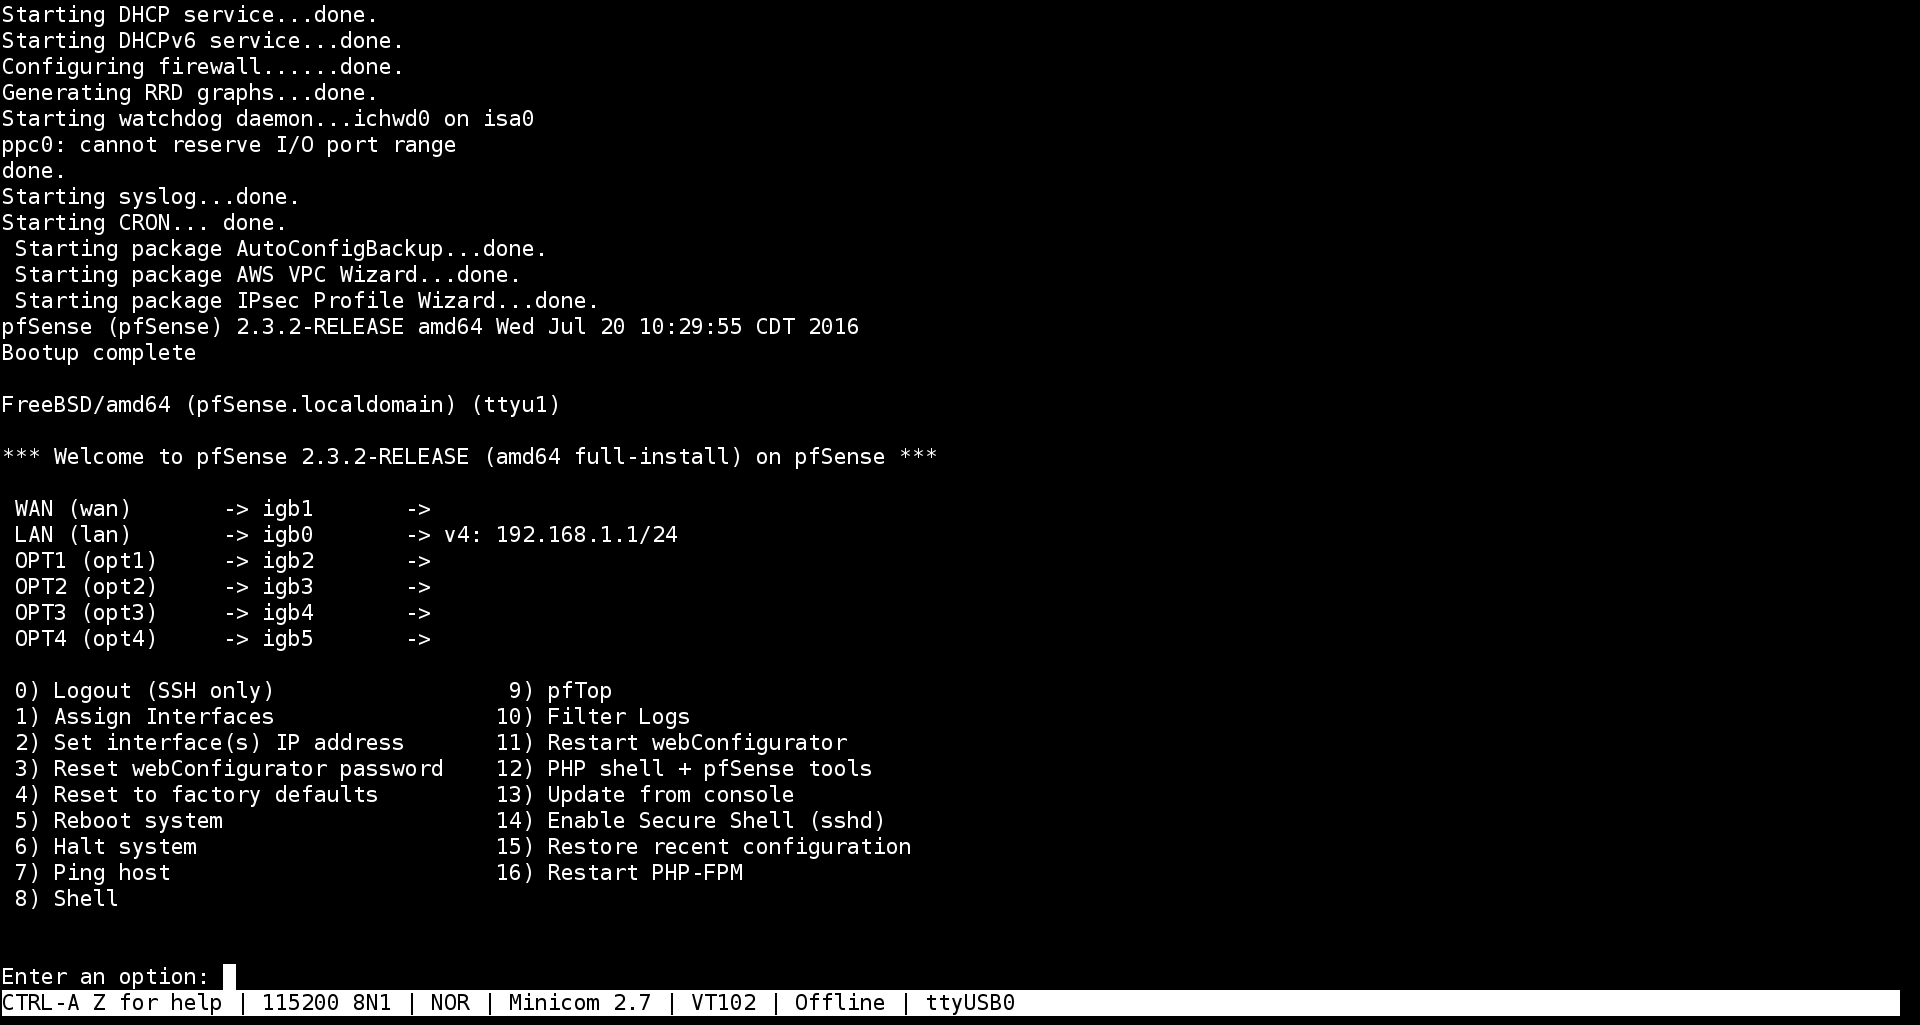
\includegraphics[keepaspectratio=true,height=0.50\textheight,width=0.75\textwidth,angle=0]{pfsense-console.png}
 \caption{pfSense Console Using \texttt{minicom}}
 \label{fig:pfsense-console}
\end{center}
\end{figure}

With the hardware all plugged in, connect with \texttt{minicom} and do some initial configuration via the USB port.
Note, it is possible to start configuration by going to \url{https://192.168.1.1} if you set an IP address on your
Debian workstation to an address in that subnet. But you won't be able to see all the bootup messages and it
will make debugging/controlling the router more difficult. With the serial connection, you can see the bootloader etc.

\begin{enumerate}
 \item Find where the USB device connected, by running \texttt{dmesg -T} on your Debian workstation.
Look for a line with USB0, USB1, etc. in it, such as:
\begin{minted}{sh}
usb 1-6: cp210x converter now attached to ttyUSB0
\end{minted}
 \item Run \texttt{minicom} on your Debian workstation to connect to the router, using the USB device from above.
 \item Your console should appear similar to figure \ref{fig:pfsense-console}.
\begin{minted}{sh}
sudo minicom -D /dev/ttyUSB0
\end{minted}

\begin{figure}[h!]
\begin{center}
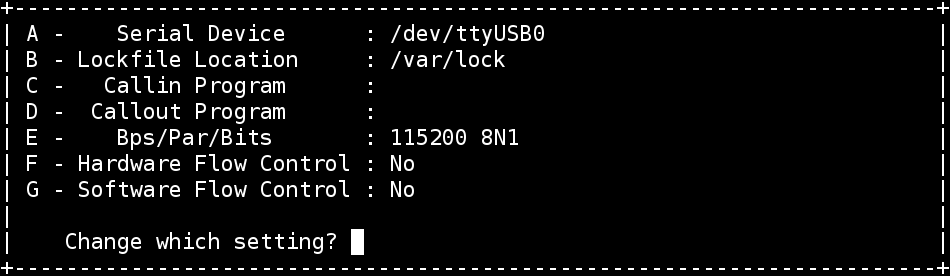
\includegraphics[keepaspectratio=true,height=0.50\textheight,width=0.75\textwidth,angle=0]{pfsense-minicom-settings.png}
 \caption{pfSense \texttt{minicom} Settings}
 \label{fig:pfsense-minicom-settings}
\end{center}
\end{figure}
 \item The connection settings are \texttt{115200 bps}, \texttt{8N1}, no \texttt{Hardware Flow Control}, no \texttt{Software Flow Control}. Note, \texttt{Hardware Flow Control} is on by default and may prevent you from entering text into the console.
 \item To change these settings in \texttt{minicom}, hit \texttt{ctrl-a} then the letter \texttt{o}.
 \item In the menu, with the arrow keys, select \texttt{Serial port setup}.
 \item Set the values listed in figure \ref{fig:pfsense-minicom-settings}.
 \item Plug in power to the pfSense router, and watch it boot up in \texttt{minicom}. It takes 1 minute, 20 seconds for a pfSense model SG-4860 firewall to cold boot with a default configuration.
 \item In the pfSense menu, select \texttt{1) Assign Interfaces}. See console listing below.
\begin{minted}[style=bw]{sh}
*** Welcome to pfSense 2.3.2-RELEASE (amd64 full-install) on pfSense ***

 WAN (wan)       -> igb1       -> 
 LAN (lan)       -> igb0       -> v4: 192.168.1.1/24
 OPT1 (opt1)     -> igb2       -> 
 OPT2 (opt2)     -> igb3       -> 
 OPT3 (opt3)     -> igb4       -> 
 OPT4 (opt4)     -> igb5       -> 

 0) Logout (SSH only)                  9) pfTop
 1) Assign Interfaces                 10) Filter Logs
 2) Set interface(s) IP address       11) Restart webConfigurator
 3) Reset webConfigurator password    12) PHP shell + pfSense tools
 4) Reset to factory defaults         13) Update from console
 5) Reboot system                     14) Enable Secure Shell (sshd)
 6) Halt system                       15) Restore recent configuration
 7) Ping host                         16) Restart PHP-FPM
 8) Shell
  
Enter an option: 1

Valid interfaces are:

igb0   00:08:a2:00:00:00   (up) Intel(R) PRO/1000 Network Connection, Version - 
igb1   00:08:a2:00:00:01 (down) Intel(R) PRO/1000 Network Connection, Version - 
igb2   00:08:a2:00:00:02 (down) Intel(R) PRO/1000 Network Connection, Version - 
igb3   00:08:a2:00:00:03 (down) Intel(R) PRO/1000 Network Connection, Version - 
igb4   00:08:a2:00:00:04 (down) Intel(R) PRO/1000 Network Connection, Version - 
igb5   00:08:a2:00:00:05 (down) Intel(R) PRO/1000 Network Connection, Version - 

Do VLANs need to be set up first?
If VLANs will not be used, or only for optional interfaces, it is typical to
say no here and use the webConfigurator to configure VLANs later, if required.

Should VLANs be set up now [y|n]? n

If the names of the interfaces are not known, auto-detection can
be used instead. To use auto-detection, please disconnect all
interfaces before pressing 'a' to begin the process.

Enter the WAN interface name or 'a' for auto-detection 
(igb0 igb1 igb2 igb3 igb4 igb5 or a): igb1

Enter the LAN interface name or 'a' for auto-detection 
NOTE: this enables full Firewalling/NAT mode.
(igb0 igb2 igb3 igb4 igb5 a or nothing if finished): igb0

Optional interface 1 description found: OPT1
Enter the Optional 1 interface name or 'a' for auto-detection
(igb2 igb3 igb4 igb5 a or nothing if finished): 

The interfaces will be assigned as follows:

WAN  -> igb1
LAN  -> igb0

Do you want to proceed [y|n]? y

Writing configuration...done.
One moment while the settings are reloading... done!
\end{minted}

 \item Note the MAC address for the LAN interface.
 \item Copy MAC address to main DHCP/DNS server, and reserve IP address. In other words, set up this new firewall on the local LAN DHCP server (if available).
 \item Set DHCP for WAN. This is assuming the WAN is on an interface with DHCP (e.g. cable modem). If it is statically set, set
the address here.
 \item Disable IPv6.
the address here.
 \item In the pfSense menu, select \texttt{2) Set interface(s) IP address},
 \item Then \texttt{1} to select the WAN interface. See console listing below.

\begin{minted}[fontsize=\scriptsize,style=bw]{sh}
Enter an option: 2

Available interfaces:

1 - WAN (igb1 - dhcp, dhcp6)
2 - LAN (igb0 - static)

Enter the number of the interface you wish to configure: 1

Configure IPv4 address WAN interface via DHCP? (y/n) y

Configure IPv6 address WAN interface via DHCP6? (y/n) n

Enter the new WAN IPv6 address.  Press <ENTER> for none:
> 

Do you want to revert to HTTP as the webConfigurator protocol? (y/n) n

Please wait while the changes are saved to WAN...
 Reloading filter...
 Reloading routing configuration...
 DHCPD...

The IPv4 WAN address has been set to dhcp

Press <ENTER> to continue.
\end{minted}

 \item Set static IP for LAN, using \texttt{10.72.9.254/24} as an example.
 \item Do not set an IPv6 address.
 \item Don't enter a gateway.
 \item Don't enable DHCP server (for now, at least).
 \item In the pfSense menu, select \texttt{2) Set interface(s) IP address}.
 \item Then \texttt{2} to select the LAN interface. See console listing below.
\begin{minted}[fontsize=\scriptsize,style=bw]{sh}
Enter an option: 2

Available interfaces:

1 - WAN (igb1 - dhcp)
2 - LAN (igb0)

Enter the number of the interface you wish to configure: 2

Enter the new LAN IPv4 address.  Press <ENTER> for none:
> 10.72.9.254

Subnet masks are entered as bit counts (as in CIDR notation) in pfSense.
e.g. 255.255.255.0 = 24
     255.255.0.0   = 16
     255.0.0.0     = 8

Enter the new LAN IPv4 subnet bit count (1 to 31):
> 24

For a WAN, enter the new LAN IPv4 upstream gateway address.
For a LAN, press <ENTER> for none:
> 

Enter the new LAN IPv6 address.  Press <ENTER> for none:
> 

Do you want to enable the DHCP server on LAN? (y/n) n

Do you want to revert to HTTP as the webConfigurator protocol? (y/n) n

Please wait while the changes are saved to LAN...
 Reloading filter...
 Reloading routing configuration...
 DHCPD...

The IPv4 LAN address has been set to 10.72.9.254/24
You can now access the webConfigurator by opening the following URL in your web browser:
                https://10.72.9.254/

Press <ENTER> to continue.
\end{minted}
\end{enumerate}

\subsection{Initial Wizard Setup via Web Browser}

\begin{enumerate}
 \item If needed, set IP address on Debian workstation that is in the same subnet as new firewall. If you have two ethernet interfaces, and the new firewall is plugged into the second ethernet interface, depending on the interface name, run one of:
\begin{minted}{sh}
ifconfig eth0 10.72.9.12
ifconfig eth1 10.72.9.12
ifconfig enp3s0 10.72.9.12
\end{minted}

If you're workstation has only one ethernet connection and the new firewall is plugged into a switch that connects to the workstation, set a second IP address on the primary ethernet interface. It will likely be this:
\begin{minted}{sh}
ifconfig eth0:0 10.72.9.12
\end{minted}

 \item On your Debian workstation, point your browser to the IP address you set on the LAN interface. For example, \url{https://10.72.9.254/}
 \item Your browser will issue a warning about the SSL certificate. Don't send to Google...

\begin{minted}[fontsize=\scriptsize,style=bw]{sh}
Your connection is not private

Attackers might be trying to steal your information from 10.72.9.254 (for example, passwords, messages, or credit cards). NET::ERR_CERT_AUTHORITY_INVALID
\end{minted}

\begin{figure}[h!]
\begin{center}
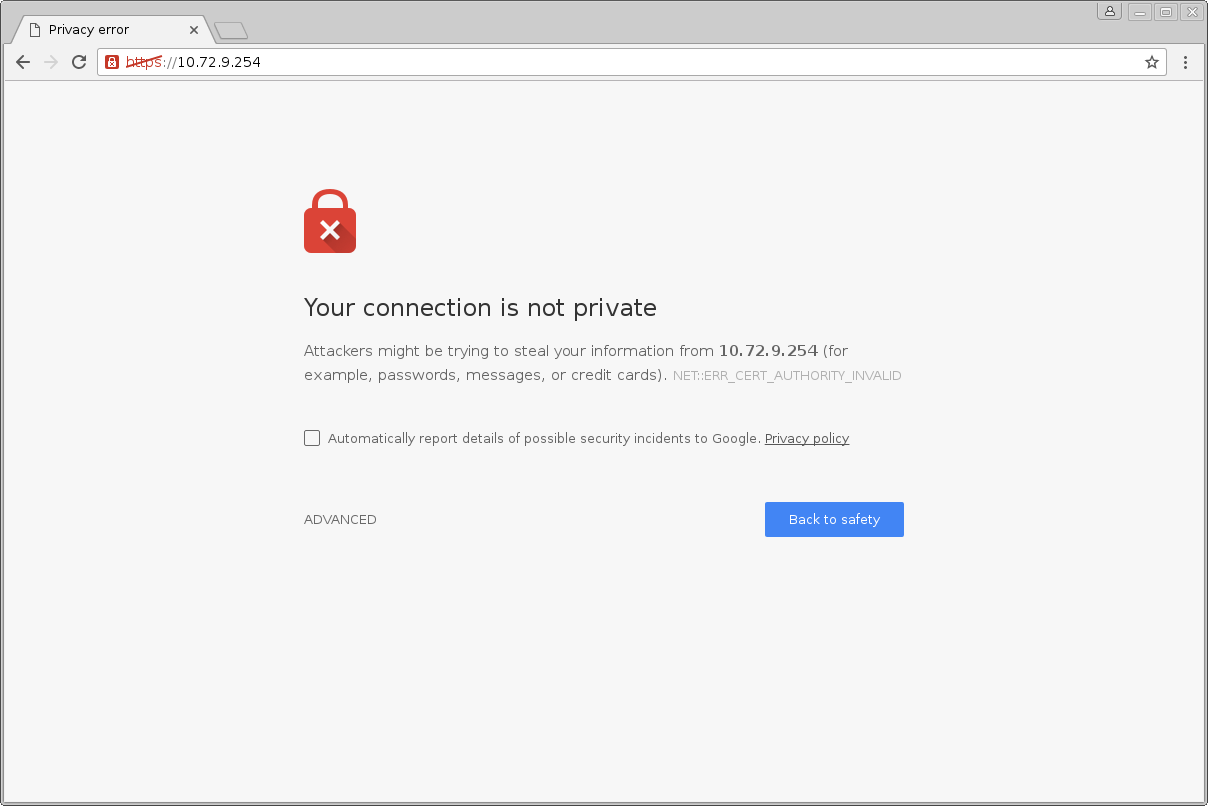
\includegraphics[keepaspectratio=true,height=0.50\textheight,width=0.75\textwidth,angle=0]{pfsense-invalidssl.png}
 \caption{pfSense Cert Authority Invalid}
 \label{fig:pfsense-invalidssl}
\end{center}
\end{figure}

 \item In your browser hit \texttt{Advanced}, which will display this text (see also figure \ref{fig:pfsense-invalidssl}:
\begin{minted}[fontsize=\scriptsize,style=bw]{sh}
This server could not prove that it is 10.72.9.254; its security certificate is not trusted by your computer's operating system. This may be caused by a misconfiguration or an attacker intercepting your connection.

Proceed to 10.72.9.254 (unsafe)
\end{minted}

 \item Click \texttt{Proceed} to go through with this operation. A new SSL cert will be set up on the firewall in later steps to replace this self-signed certificate.

 \item Log in to firewall (e.g. \url{https://10.72.9.254}). The initial username is \texttt{admin} and the password is \texttt{pfsense}, as seen in figure \ref{fig:pfsense-long}.

\begin{figure}[h!]
\begin{center}
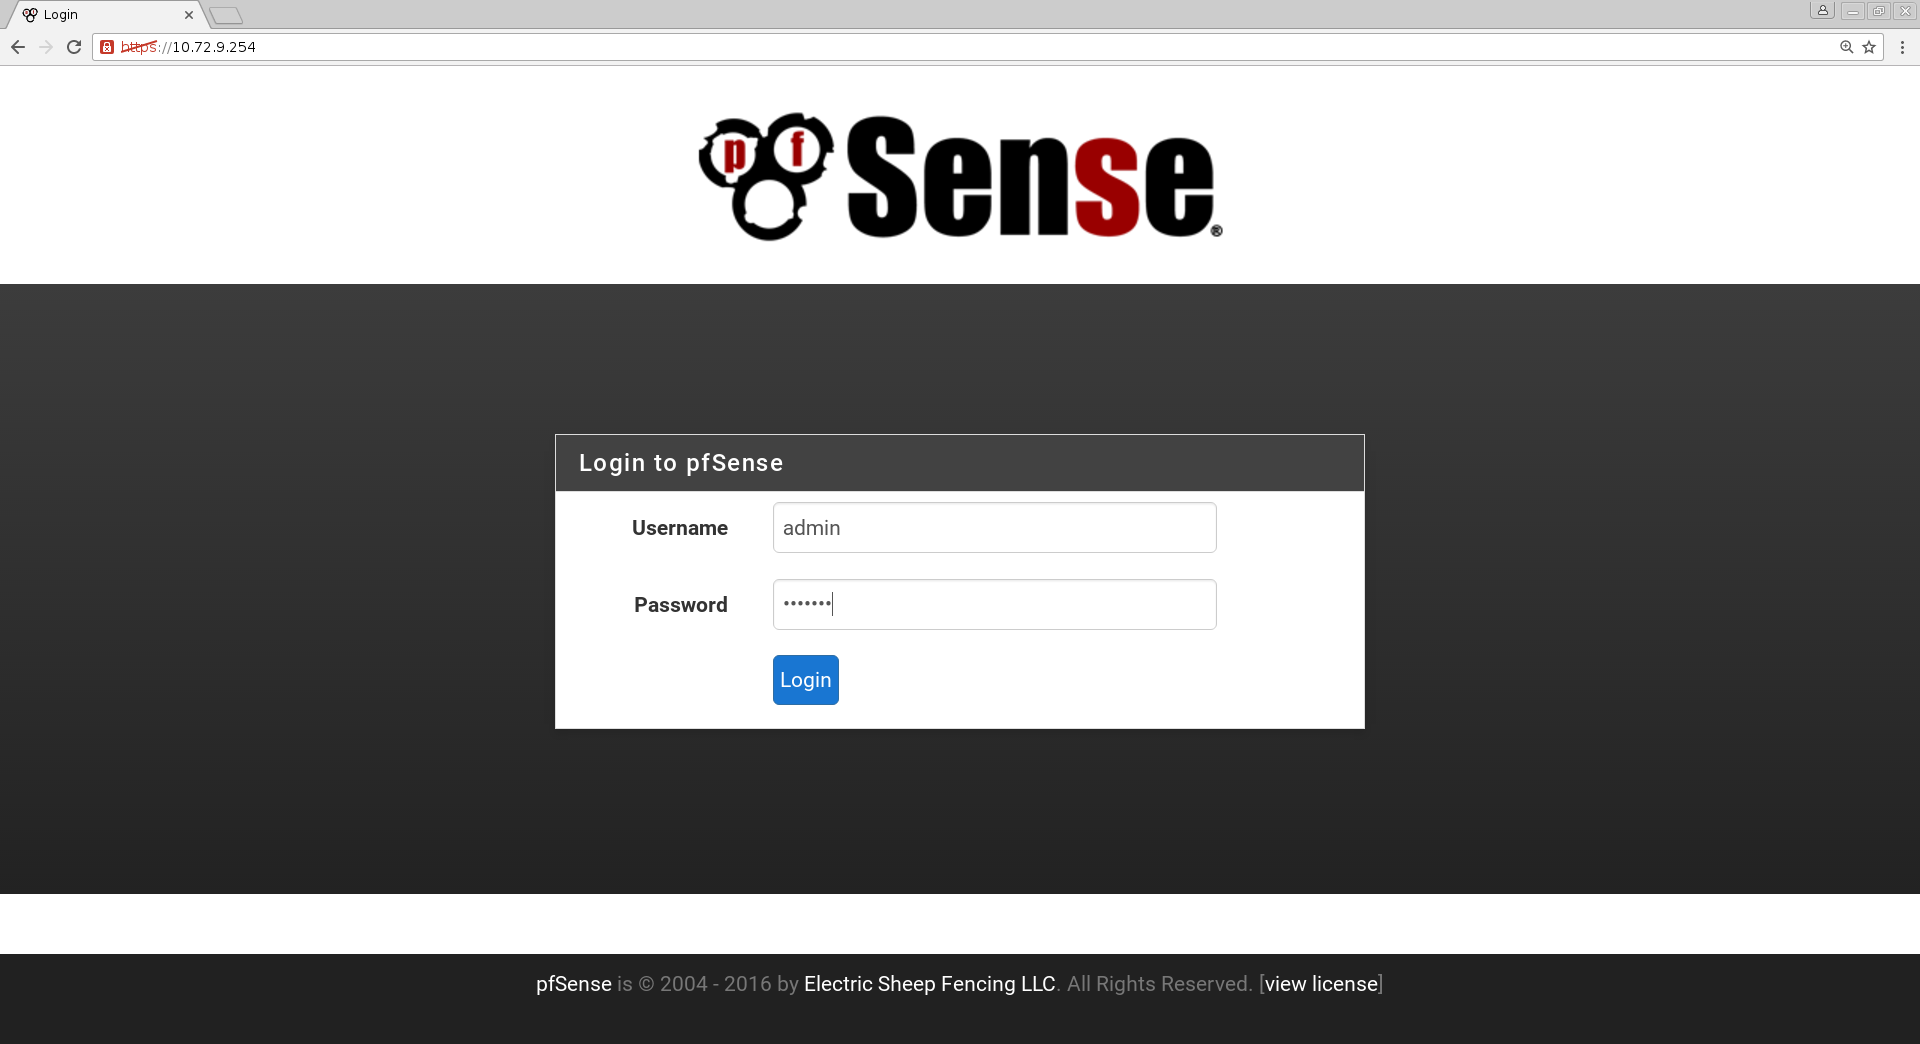
\includegraphics[keepaspectratio=true,height=0.50\textheight,width=0.75\textwidth,angle=0]{pfsense-login.png}
 \caption{pfSense Login}
 \label{fig:pfsense-login}
\end{center}
\end{figure}

 \item Start Wizard (figure \ref{fig:pfsense-wizard-01}), hit \texttt{Next}.

\begin{figure}[h!]
\begin{center}
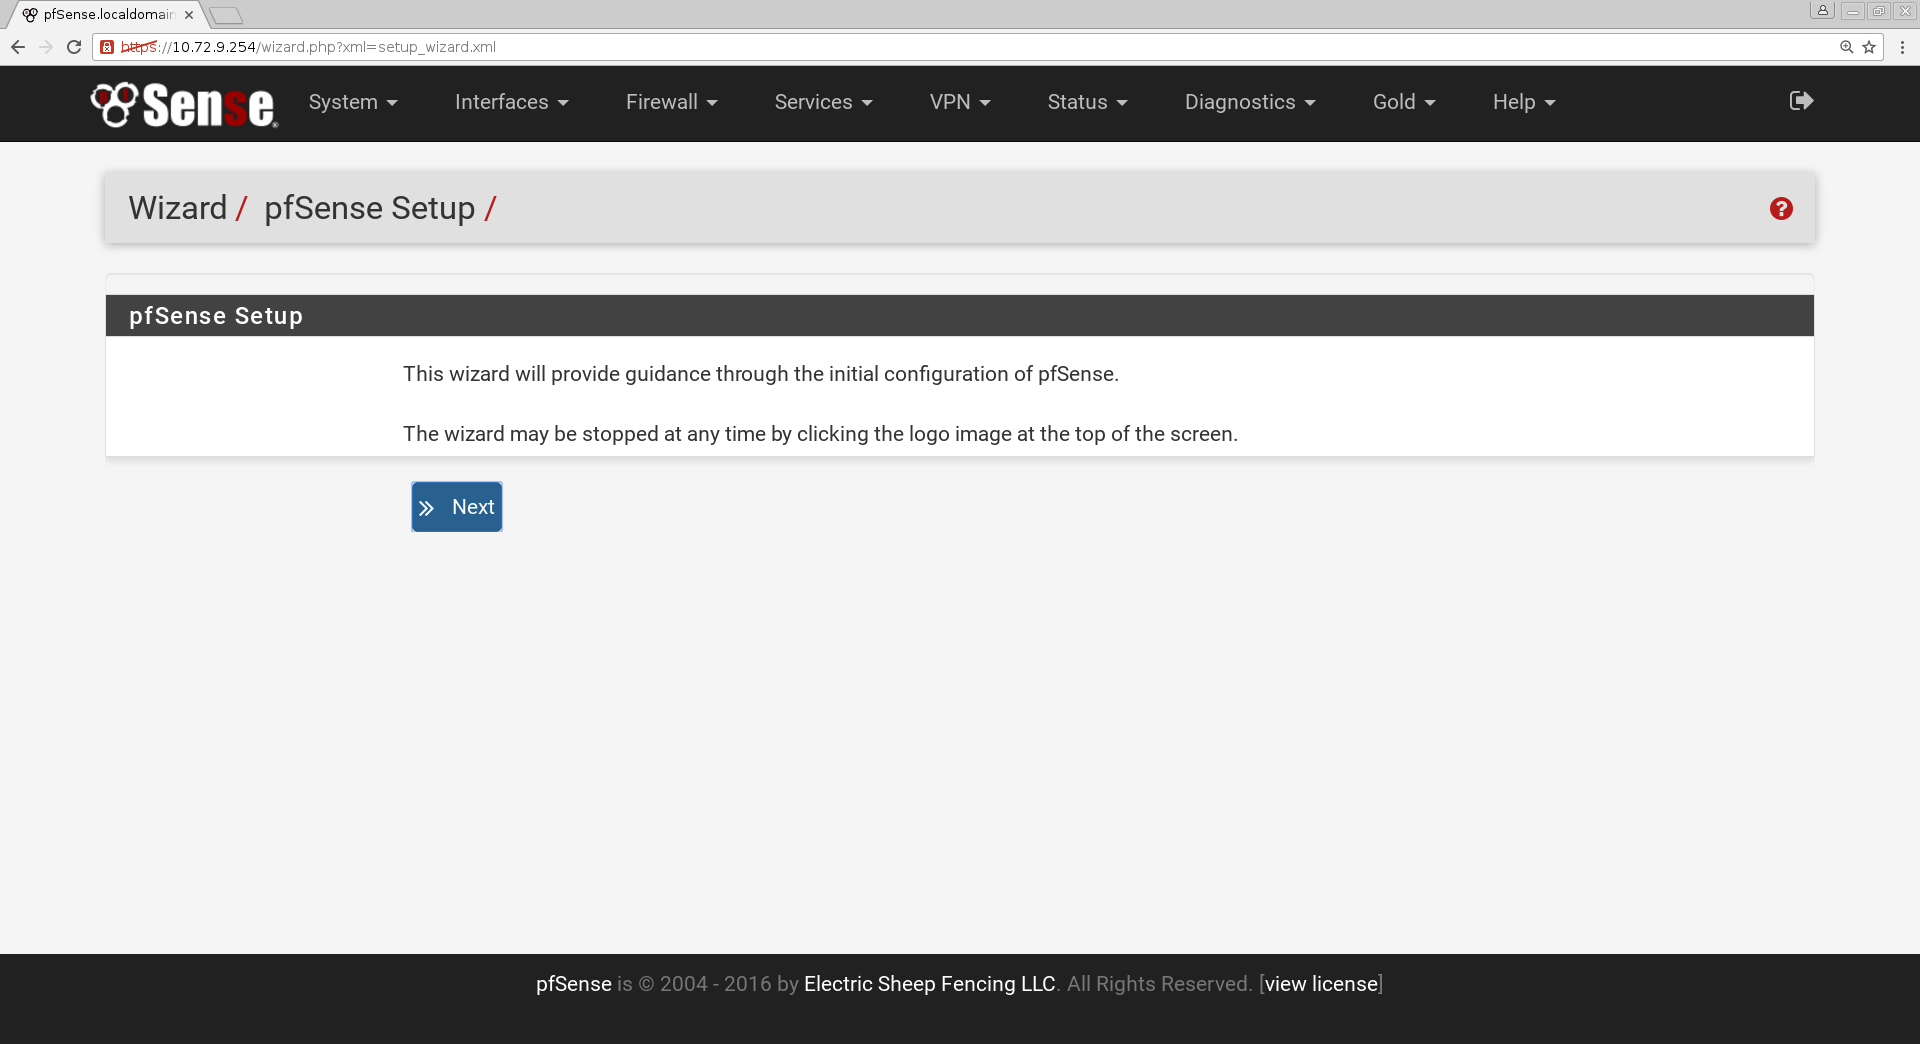
\includegraphics[keepaspectratio=true,height=0.50\textheight,width=0.75\textwidth,angle=0]{pfsense-wizard-01.png}
 \caption{pfSense Wizard}
 \label{fig:pfsense-wizard-01}
\end{center}
\end{figure}

 \item pfSense Gold plea, see (figure \ref{fig:pfsense-wizard-02}), hit \texttt{Next}.

\begin{figure}[h!]
\begin{center}
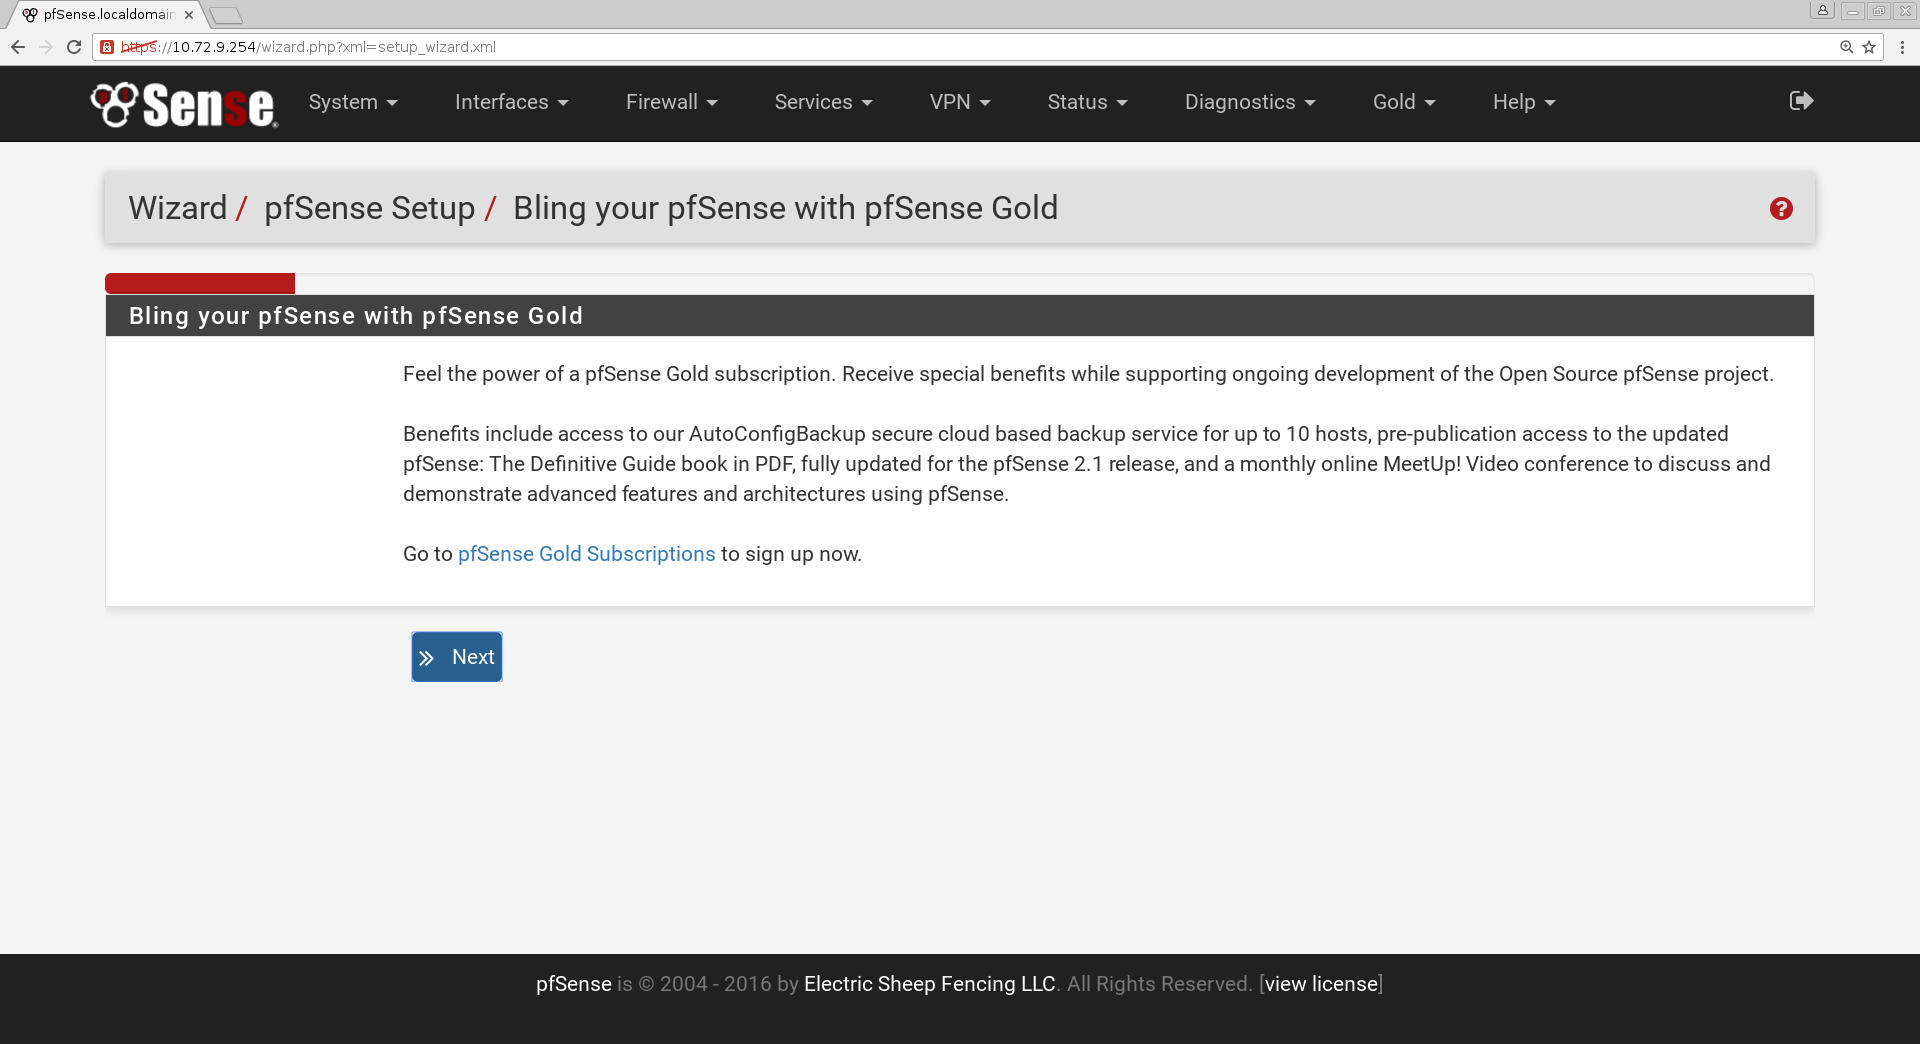
\includegraphics[keepaspectratio=true,height=0.50\textheight,width=0.75\textwidth,angle=0]{pfsense-wizard-02.png}
 \caption{pfSense Gold}
 \label{fig:pfsense-wizard-02}
\end{center}
\end{figure}

\begin{figure}[h!]
\begin{center}
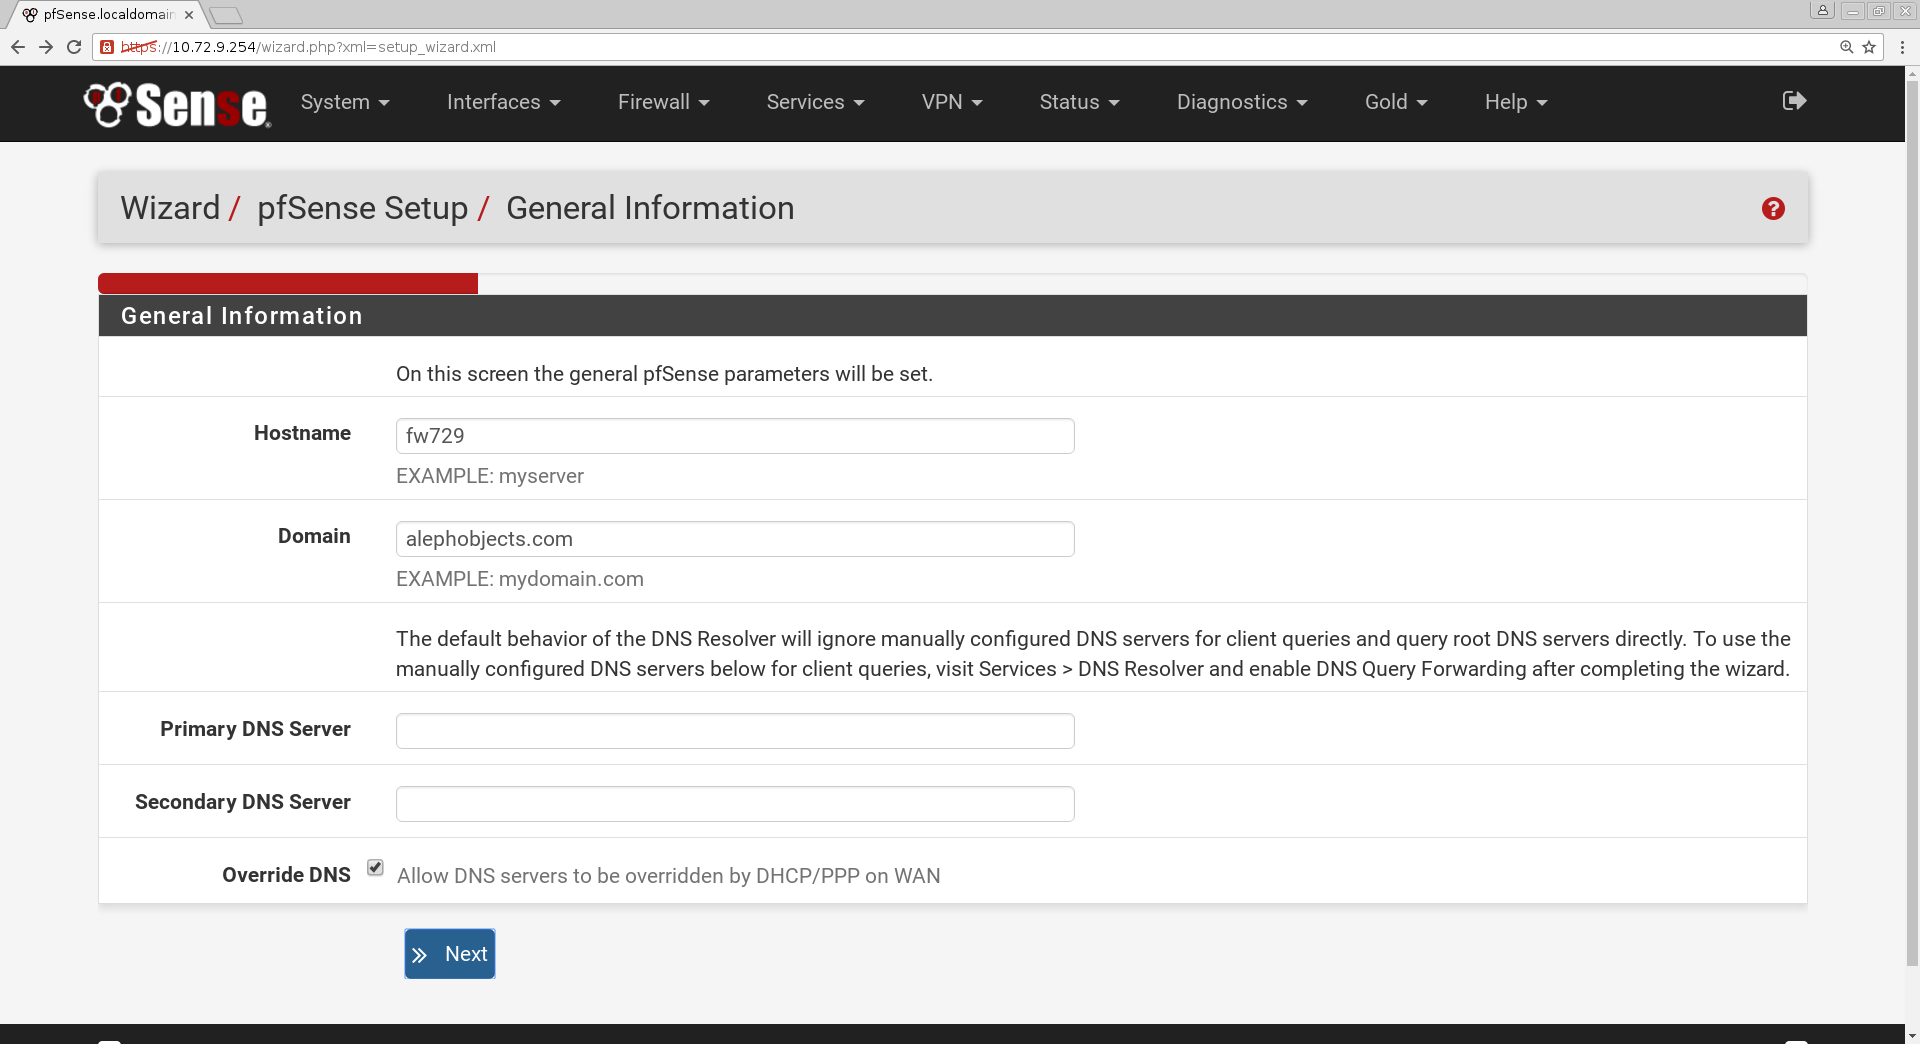
\includegraphics[keepaspectratio=true,height=0.50\textheight,width=0.75\textwidth,angle=0]{pfsense-wizard-03.png}
 \caption{pfSense Wizard General Information}
 \label{fig:pfsense-wizard-03}
\end{center}
\end{figure}

 \item This is the \texttt{General Information} page of the wizard, see figure \ref{fig:pfsense-wizard-03}.
 \item Set \texttt{Hostname}, in this example \texttt{fw729}. Select a different hostname than \texttt{fw729}.
 \item Set \texttt{Domain}, in this example \texttt{alephobjects.com}.
 \item \texttt{Primary DNS Server} and \texttt{Secondary DNS Server} can be blank for now. They will be set it later steps.
 \item \texttt{Override DNS}, leave checked.
 \item Hit \texttt{Next} to save.

\begin{figure}[h!]
\begin{center}
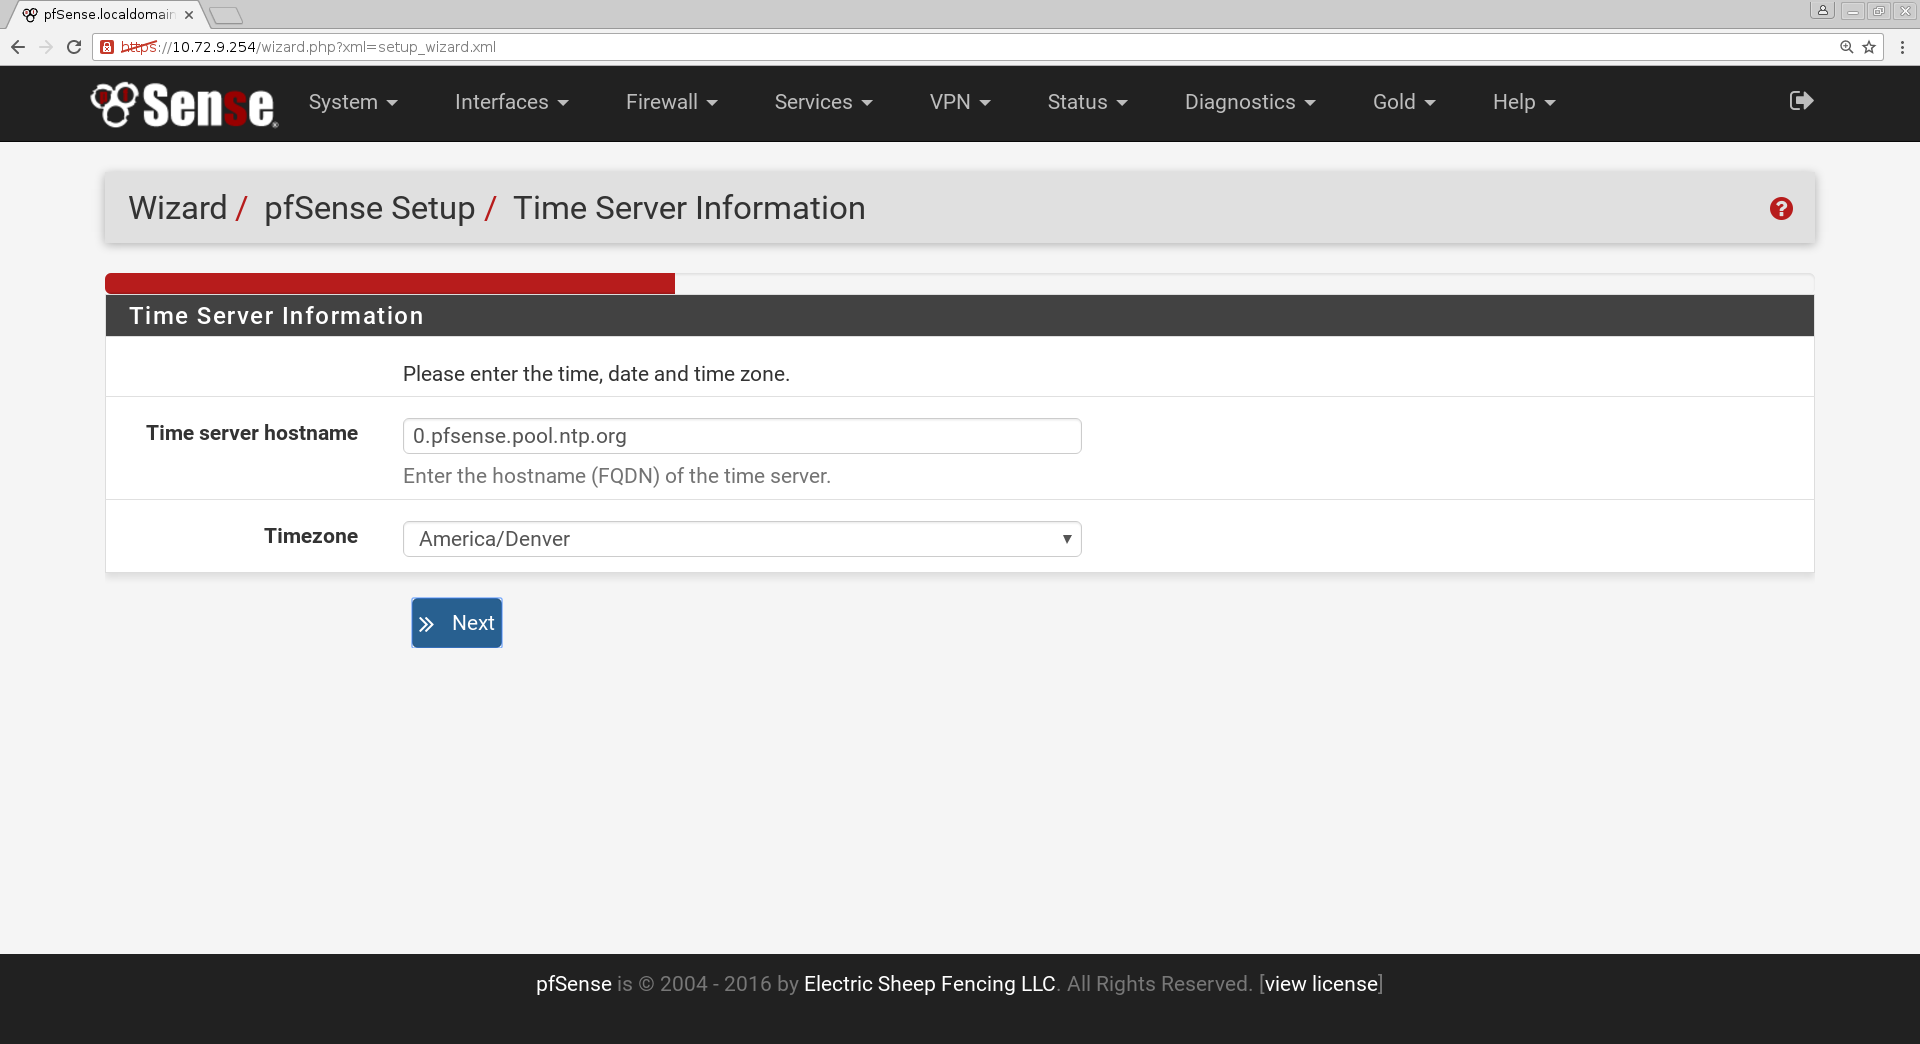
\includegraphics[keepaspectratio=true,height=0.50\textheight,width=0.75\textwidth,angle=0]{pfsense-wizard-04.png}
 \caption{pfSense Wizard Timezone}
 \label{fig:pfsense-wizard-04}
\end{center}
\end{figure}

 \item The \texttt{Time Server Information} page of the wizard, see figure \ref{fig:pfsense-wizard-04}.
 \item \texttt{Time Server Hostname}, leave at default.
 \item Set \texttt{Timezone} to \texttt{America/Denver}.
 \item Hit \texttt{Next} to save.

\begin{figure}[h!]
\begin{center}
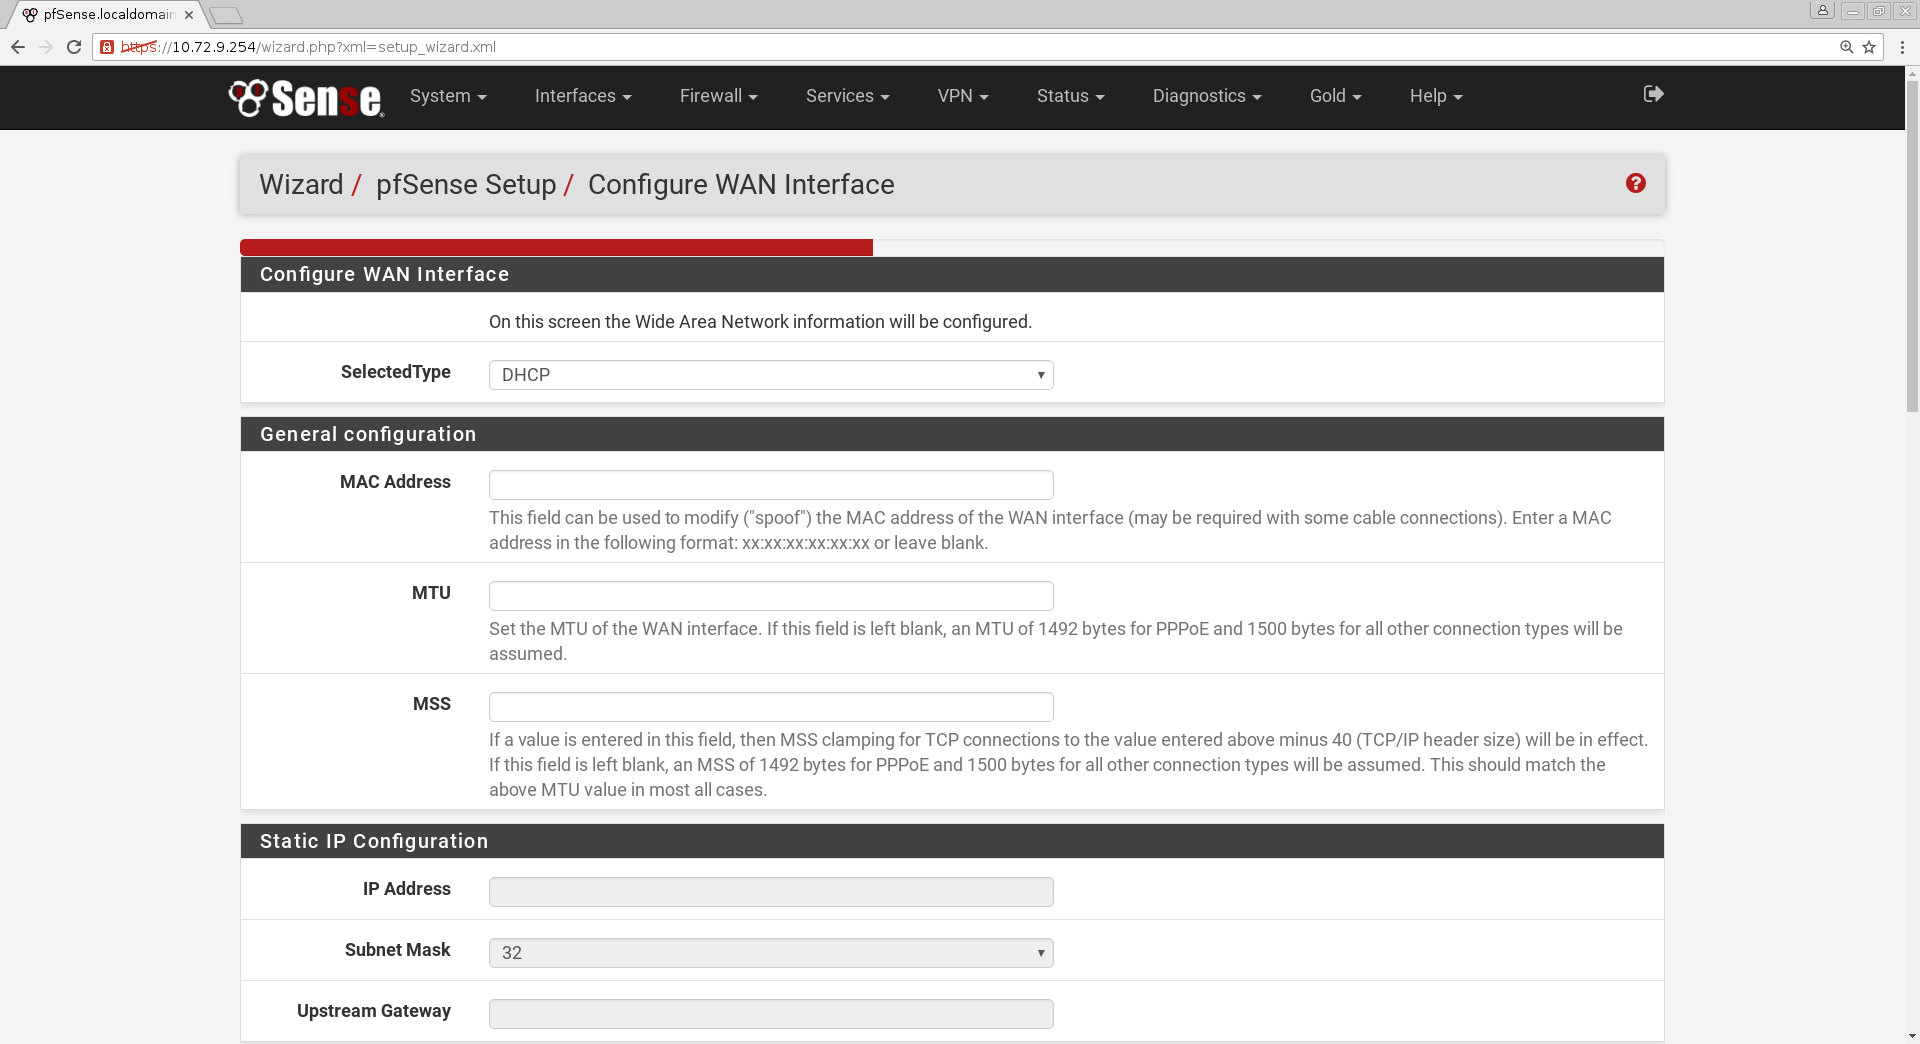
\includegraphics[keepaspectratio=true,height=0.50\textheight,width=0.75\textwidth,angle=0]{pfsense-wizard-05.png}
 \caption{pfSense Wizard WAN Configuration}
 \label{fig:pfsense-wizard-05}
\end{center}
\end{figure}

 \item The \texttt{Configure WAN Interface} page of the wizard, see figure \ref{fig:pfsense-wizard-05}.
 \item Configure WAN interface. Leave the WAN interface ethernet cable unplugged. In later steps, once we get the basic firewalling etc. running, we can plug in WAN and configure it. For now, take the WAN DHCP defaults.
 \item See figure \ref{fig:pfsense-wizard-05}.
 \item \texttt{Selected type} use \texttt{DHCP}.
 \item \texttt{MAC Address}, leave blank.
 \item \texttt{MTU}, leave blank.
 \item \texttt{MSS}, leave blank.
 \item \texttt{MAC Address}, leave blank.
 \item Hit \texttt{Next} to save.

 \item Configure LAN interface.
\begin{figure}[h!]
\begin{center}
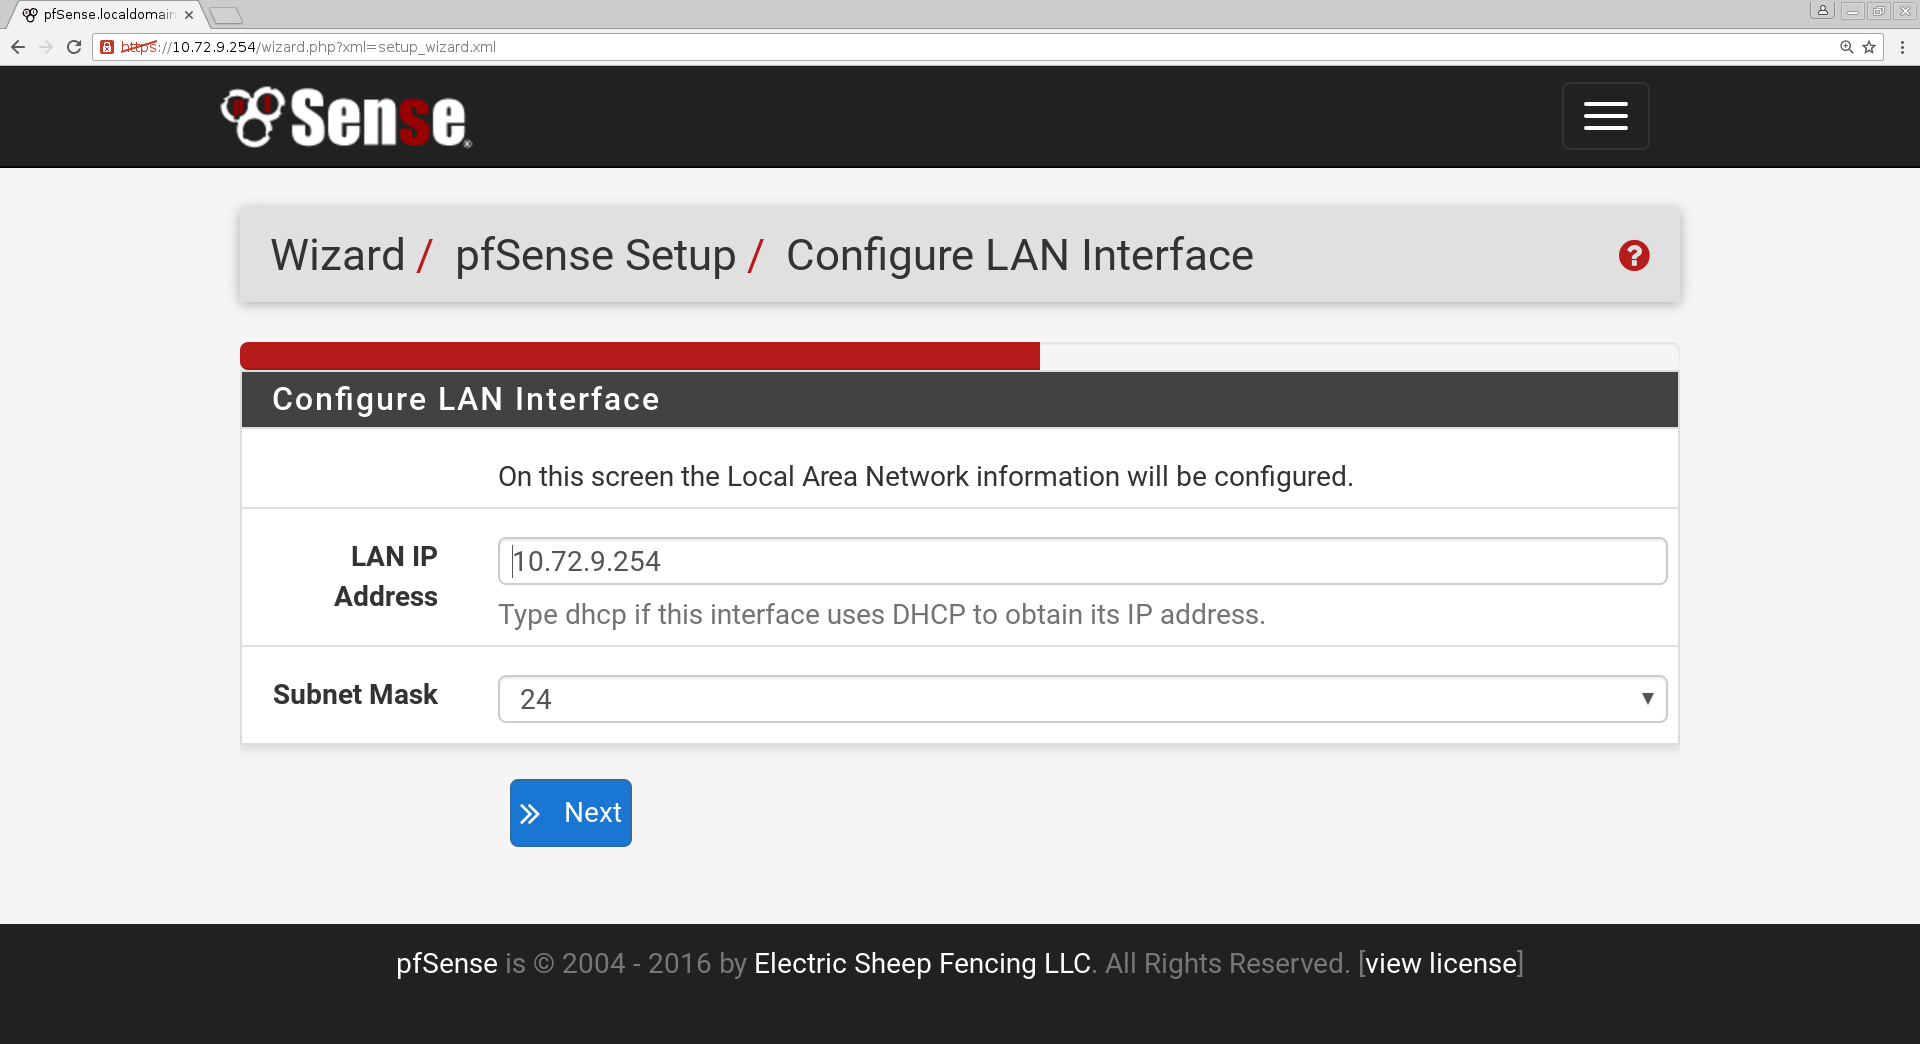
\includegraphics[keepaspectratio=true,height=0.50\textheight,width=0.75\textwidth,angle=0]{pfsense-wizard-06.png}
 \caption{pfSense Wizard LAN Configuration}
 \label{fig:pfsense-wizard-06}
\end{center}
\end{figure}

 \item The \texttt{Configure LAN Interface} page of the wizard, see figure \ref{fig:pfsense-wizard-06}.
 \item \texttt{LAN IP Address}, set the static IP. In this example \texttt{10.72.9.254}.
 \item \texttt{Subnet Mask}, set to \texttt{24}, which is \texttt{255.255.255.0}.
 \item Hit \texttt{Next} to save.

 \item \texttt{Set Admin WebGUI Password}, see figure \ref{fig:pfsense-wizard-07}.
 \item Choose something unique and following good practices. Use a good password generator.
\begin{figure}[h!]
\begin{center}
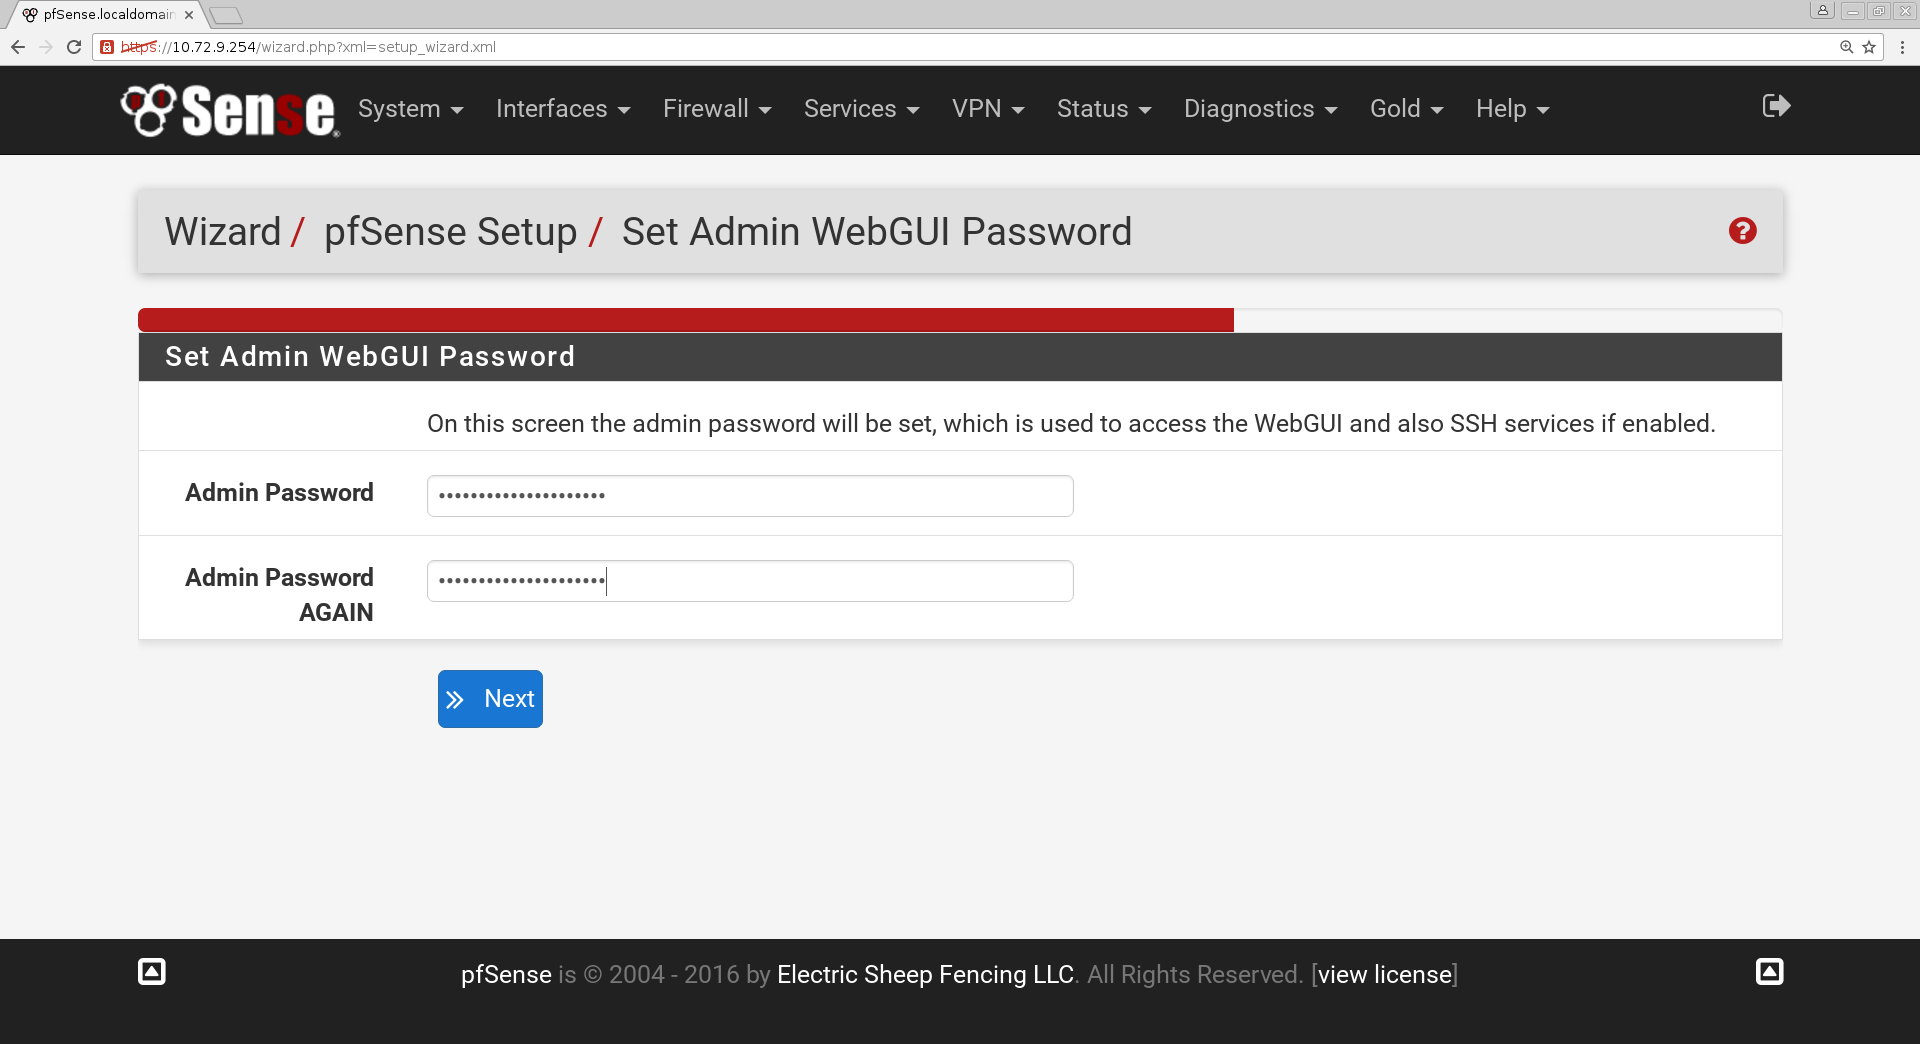
\includegraphics[keepaspectratio=true,height=0.50\textheight,width=0.75\textwidth,angle=0]{pfsense-wizard-07.png}
 \caption{pfSense Wizard Admin Password}
 \label{fig:pfsense-wizard-07}
\end{center}
\end{figure}
 \item Hit \texttt{Next} to save.

 \item Hit \texttt{Reload} to use the new configuration.
\begin{figure}[h!]
\begin{center}
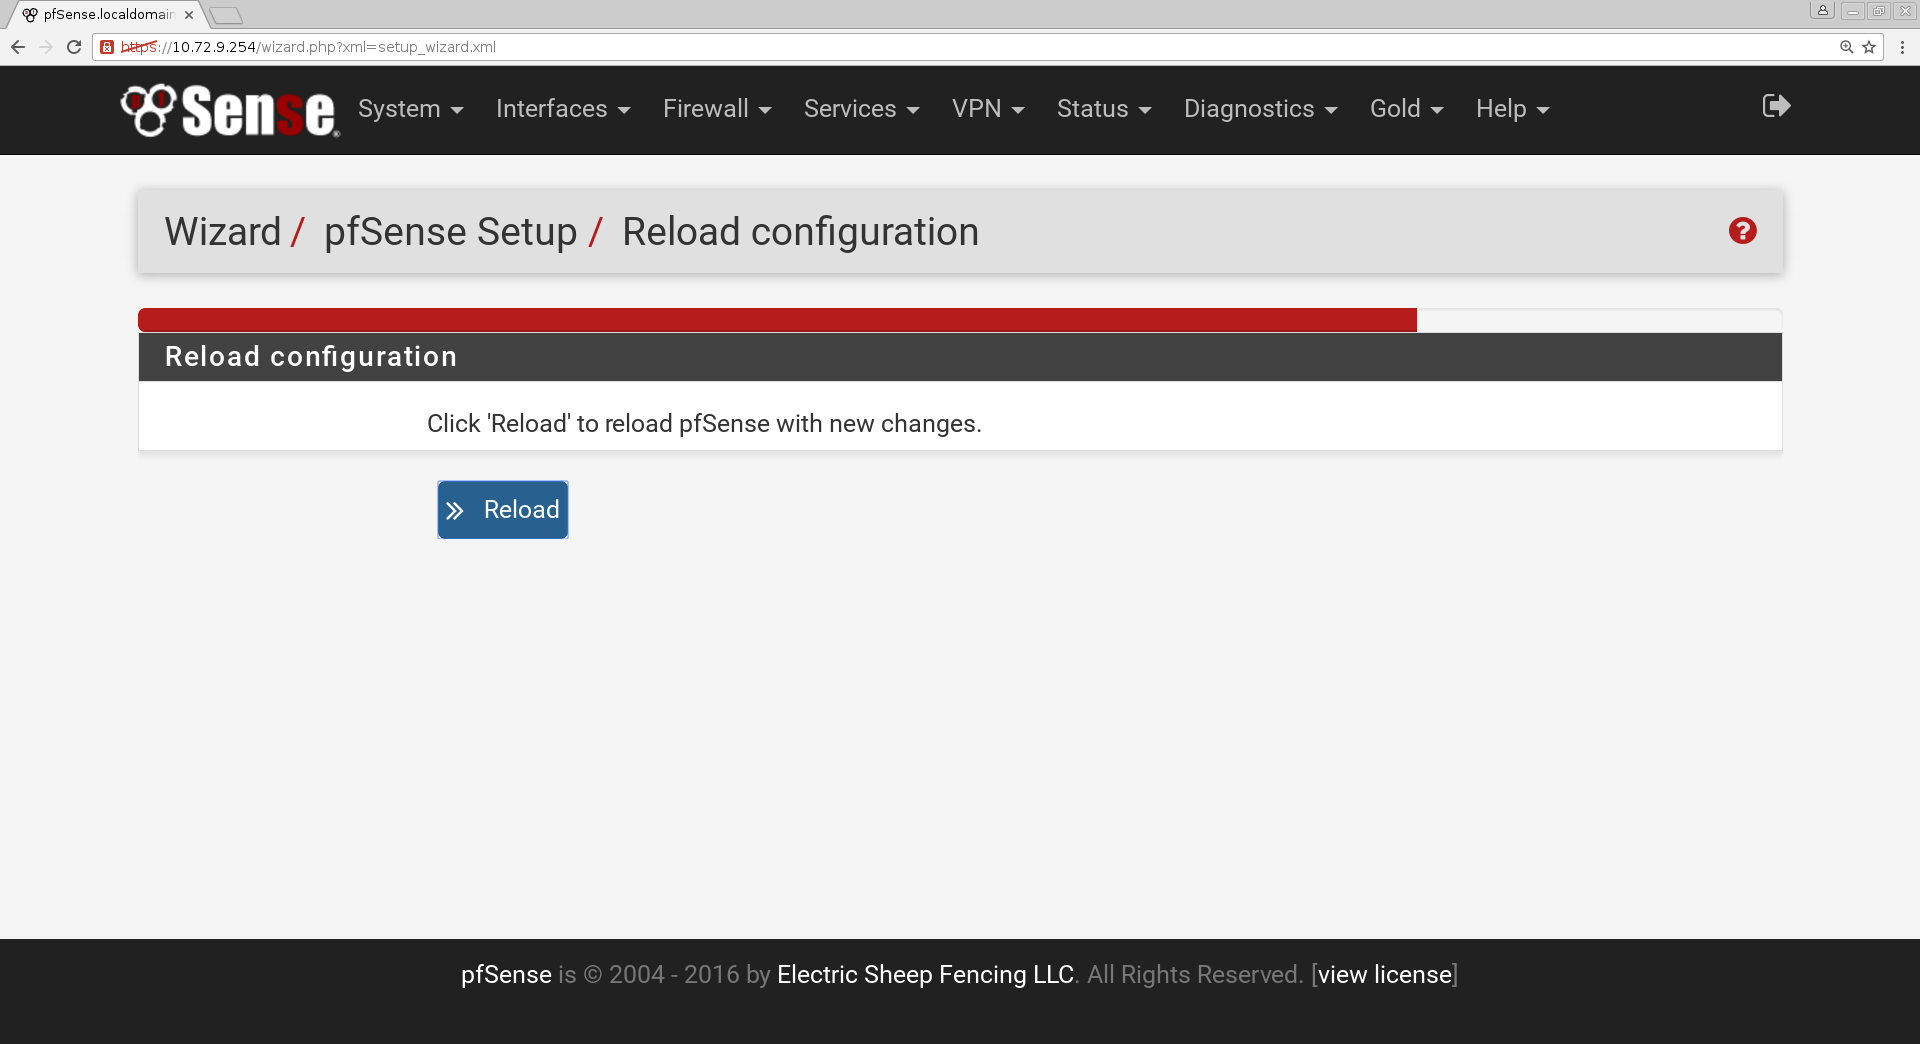
\includegraphics[keepaspectratio=true,height=0.50\textheight,width=0.75\textwidth,angle=0]{pfsense-wizard-08.png}
 \caption{pfSense Wizard Reload Configuration}
 \label{fig:pfsense-wizard-08}
\end{center}
\end{figure}

 \item Watch wizard reload. This should take less than a minute.
\begin{figure}[h!]
\begin{center}
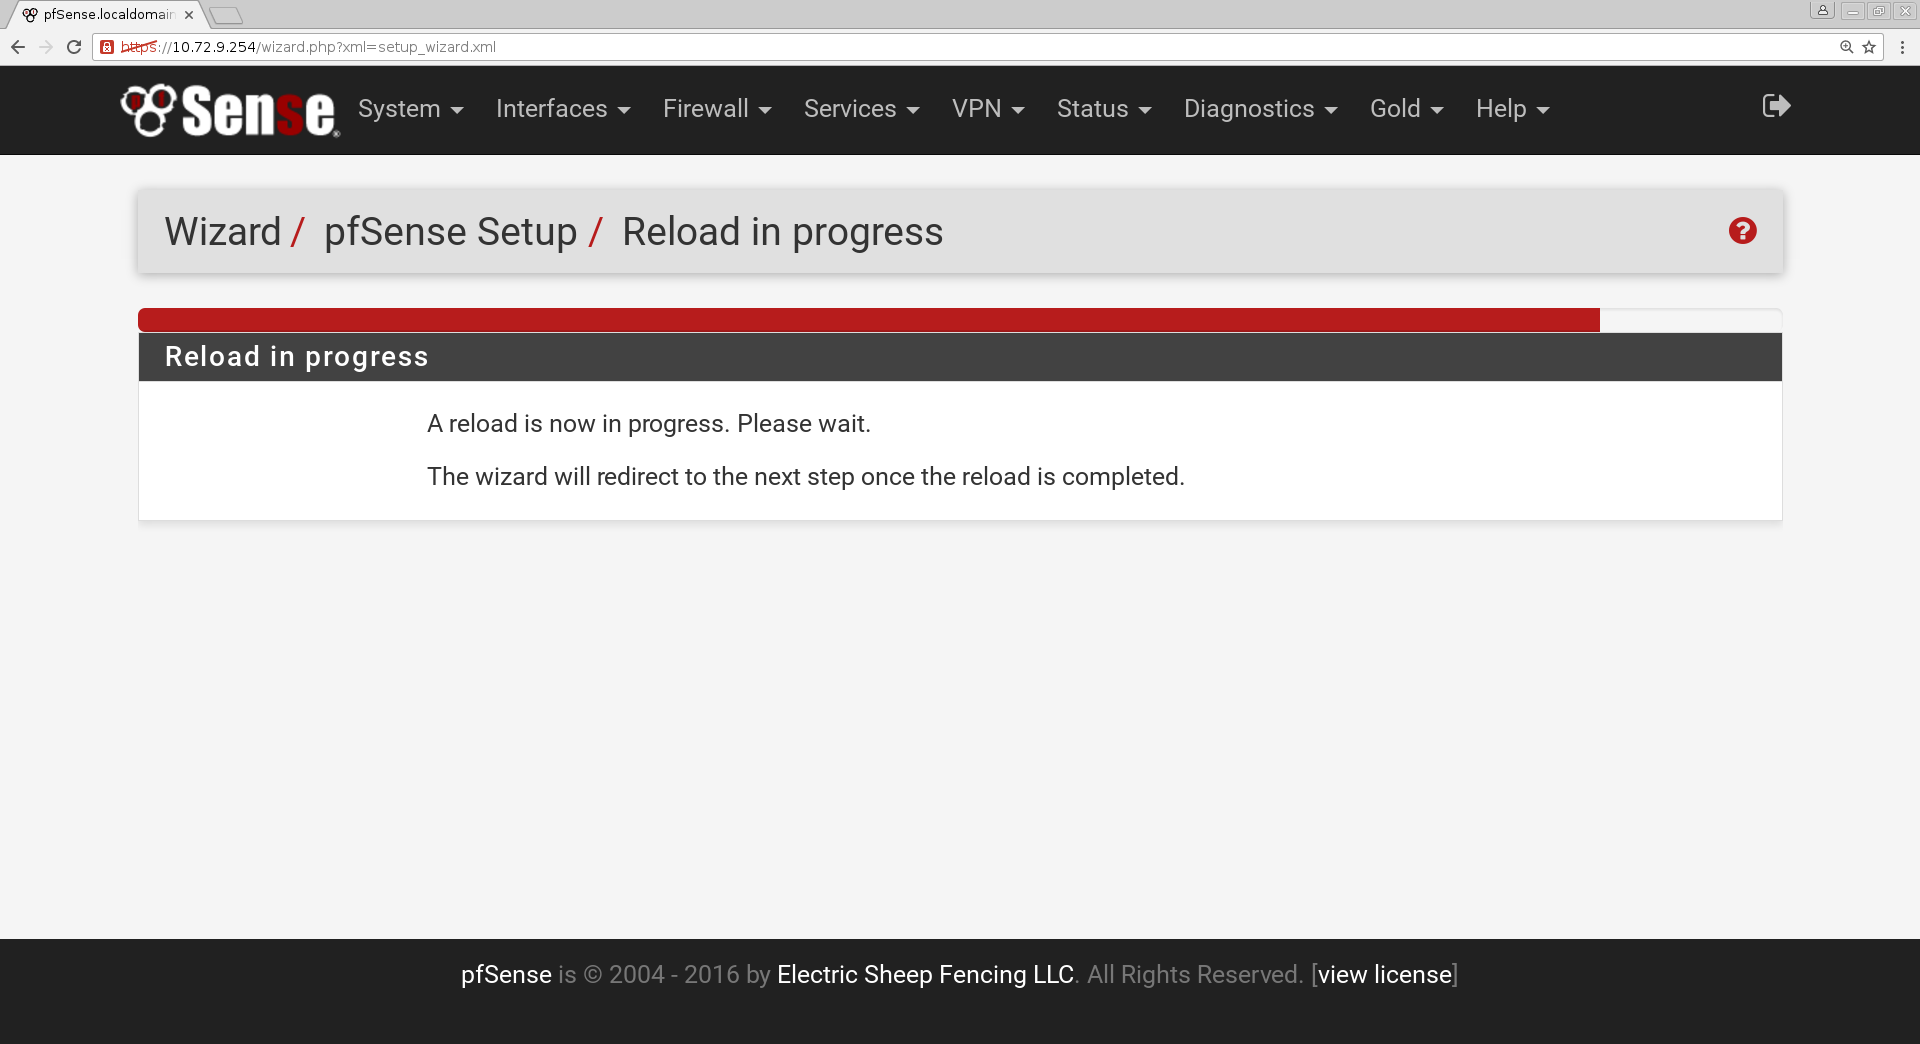
\includegraphics[keepaspectratio=true,height=0.50\textheight,width=0.75\textwidth,angle=0]{pfsense-wizard-09.png}
 \caption{pfSense Wizard Reloading}
 \label{fig:pfsense-wizard-09}
\end{center}
\end{figure}

 \item The wizard is now complete. Click \texttt{here} in \texttt{Click here to continue on to pfSense webConfigurator.}
\begin{figure}[h!]
\begin{center}
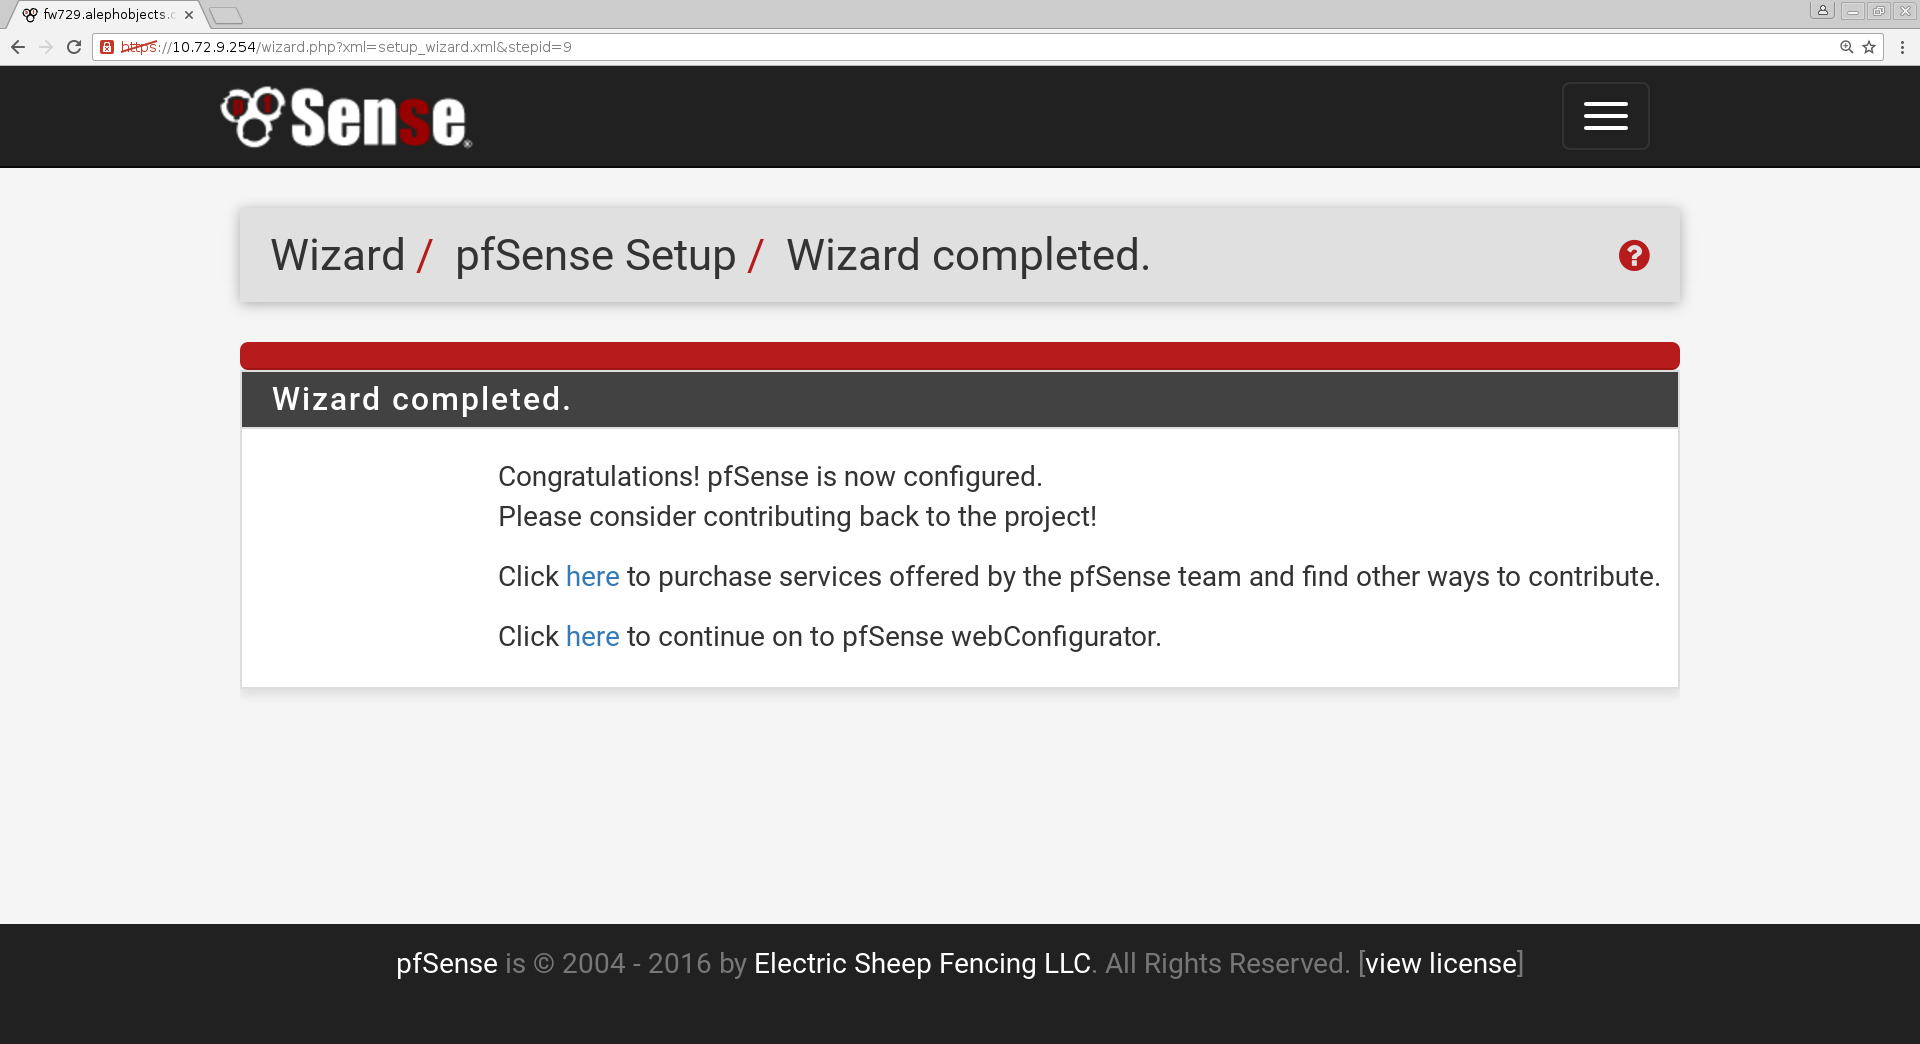
\includegraphics[keepaspectratio=true,height=0.50\textheight,width=0.75\textwidth,angle=0]{pfsense-wizard-10.png}
 \caption{pfSense Wizard Complete}
 \label{fig:pfsense-wizard-10}
\end{center}
\end{figure}

\end{enumerate}

\subsection{Initial Dashboard}
\begin{figure}[h!]
\begin{center}
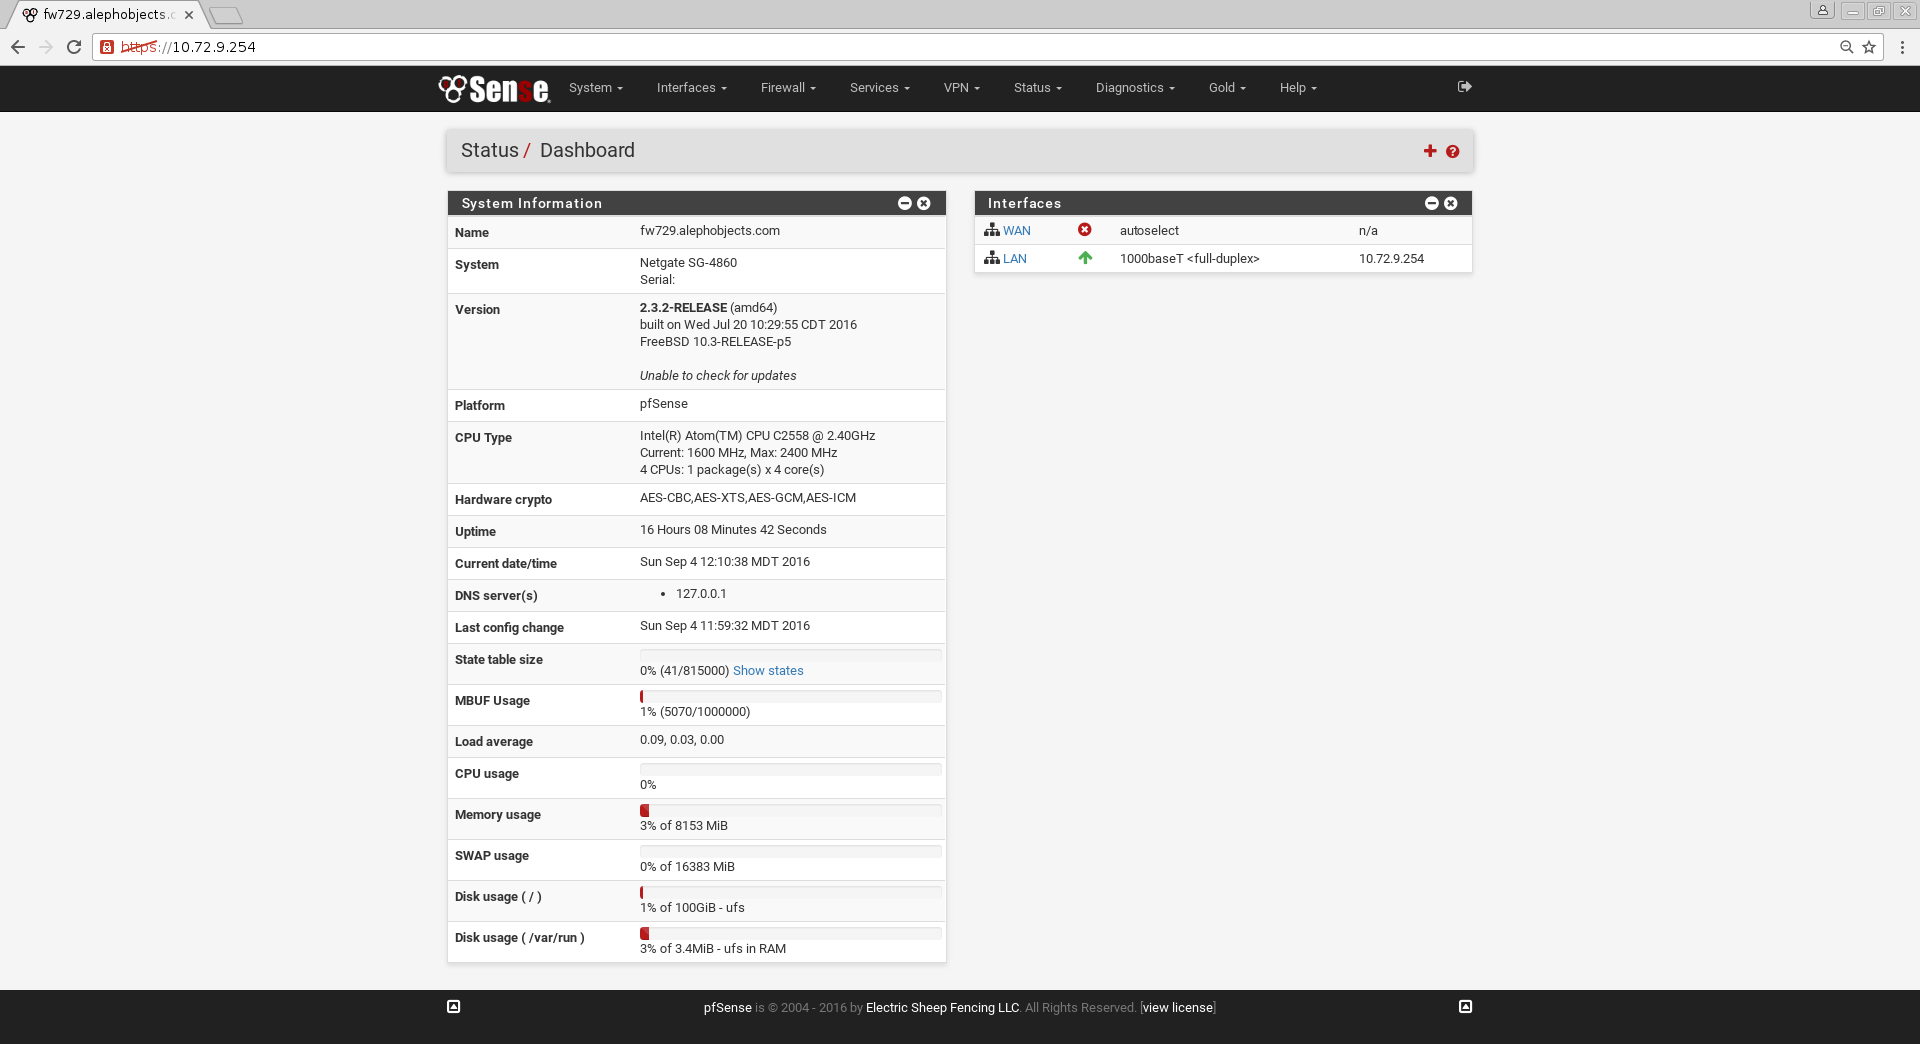
\includegraphics[keepaspectratio=true,height=0.50\textheight,width=0.75\textwidth,angle=0]{pfsense-dashboard-01.png}
 \caption{pfSense Initial Dashboard}
 \label{fig:pfsense-dashboard-01}
\end{center}
\end{figure}

The main dashboard gives an overview of the system. It will be configured more in later steps.


\subsection{Moar Configuration}
Now that the basic setup of the firewall is done...there is more...
Upon logging in the first time, you are greeted with a basic Dashboard. Menu items are across the top.

\subsection{Set Up a New User}
%\begin{figure}[h!]
%\begin{center}
%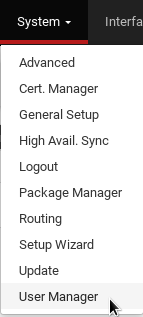
\includegraphics[keepaspectratio=true,height=0.15\textheight,width=0.15\textwidth,angle=0]{pfsense-menu-system-user.png}
% \caption{pfSense Menu, System User Manager}
% \label{fig:pfsense-menu-system-user}
%\end{center}
%\end{figure}

\begin{enumerate}
 \item Go to the top \texttt{System} tab and click \texttt{User Manager}.
\begin{figure}[h!]
\begin{center}
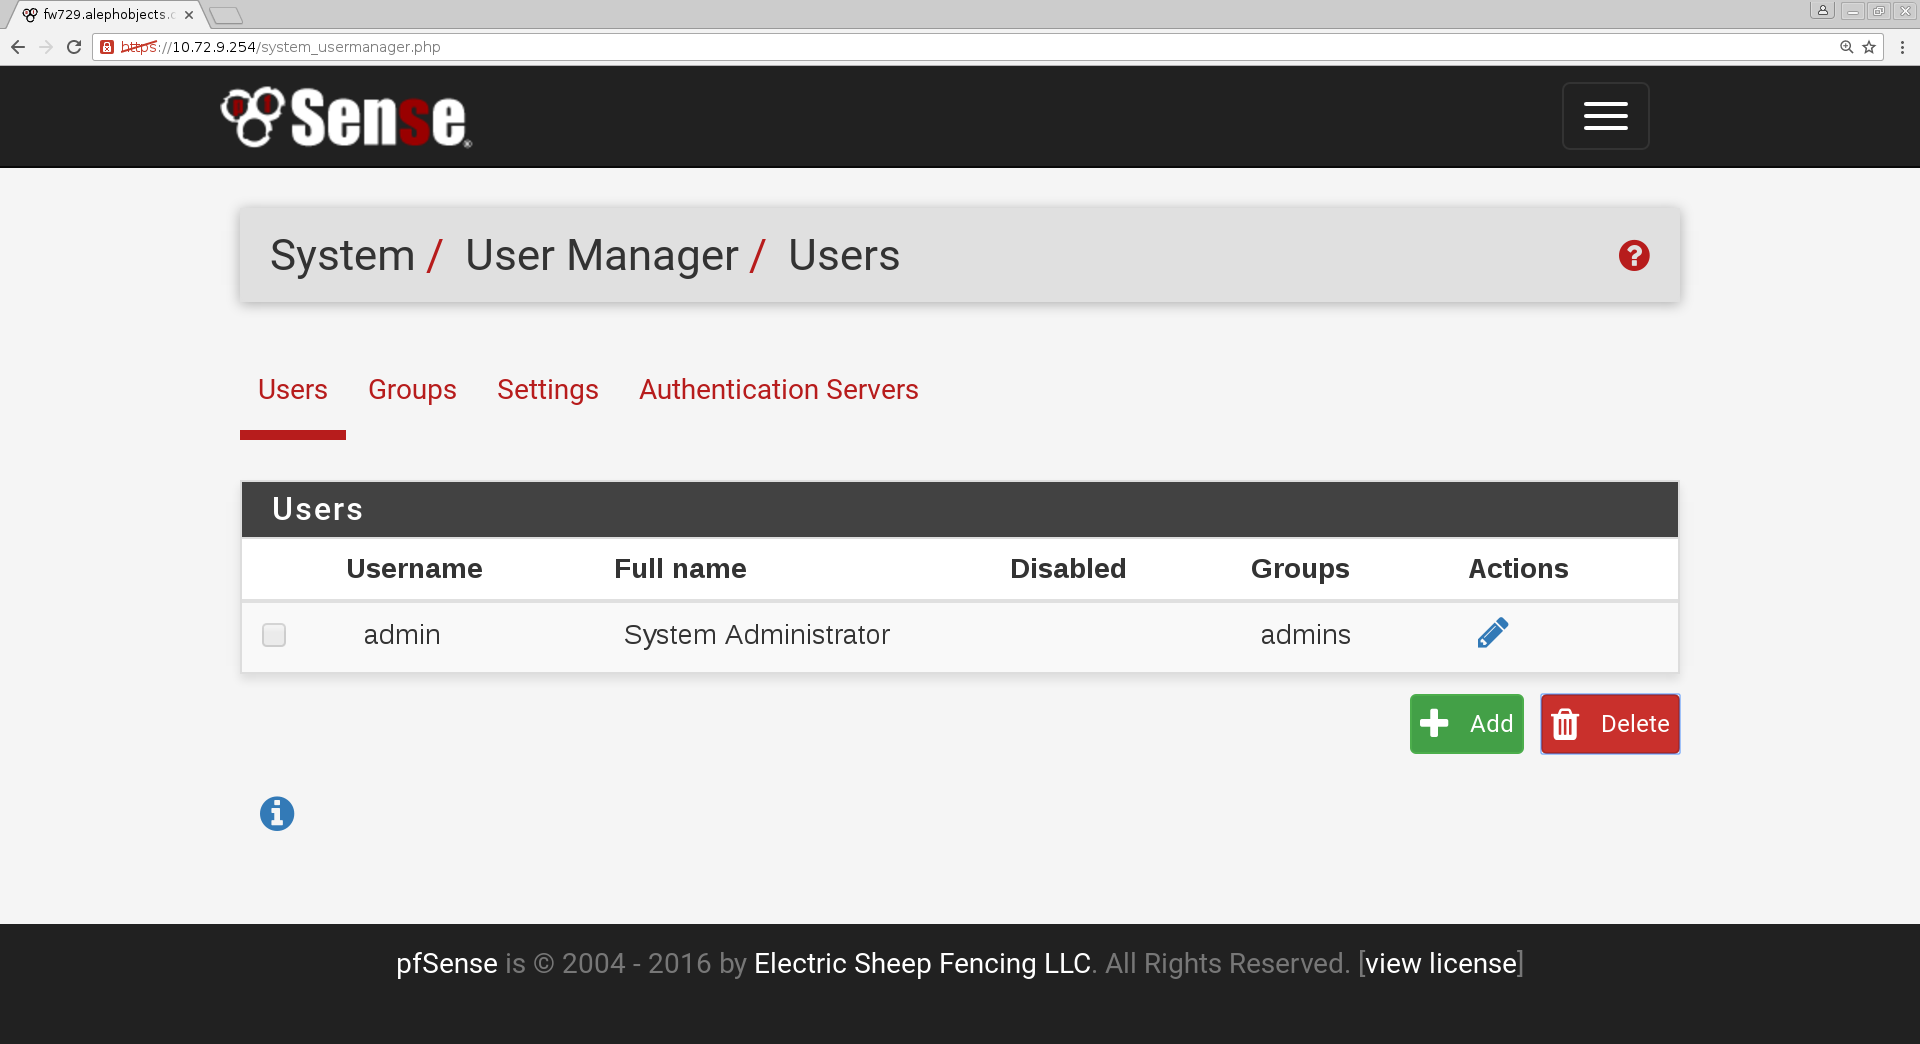
\includegraphics[keepaspectratio=true,height=0.50\textheight,width=0.75\textwidth,angle=0]{pfsense-system-user-users.png}
 \caption{pfSense Menu: System, User Manager, Users}
 \label{fig:pfsense-system-user-users}
\end{center}
\end{figure}

 \item Click Add.

\begin{figure}[h!]
\begin{center}
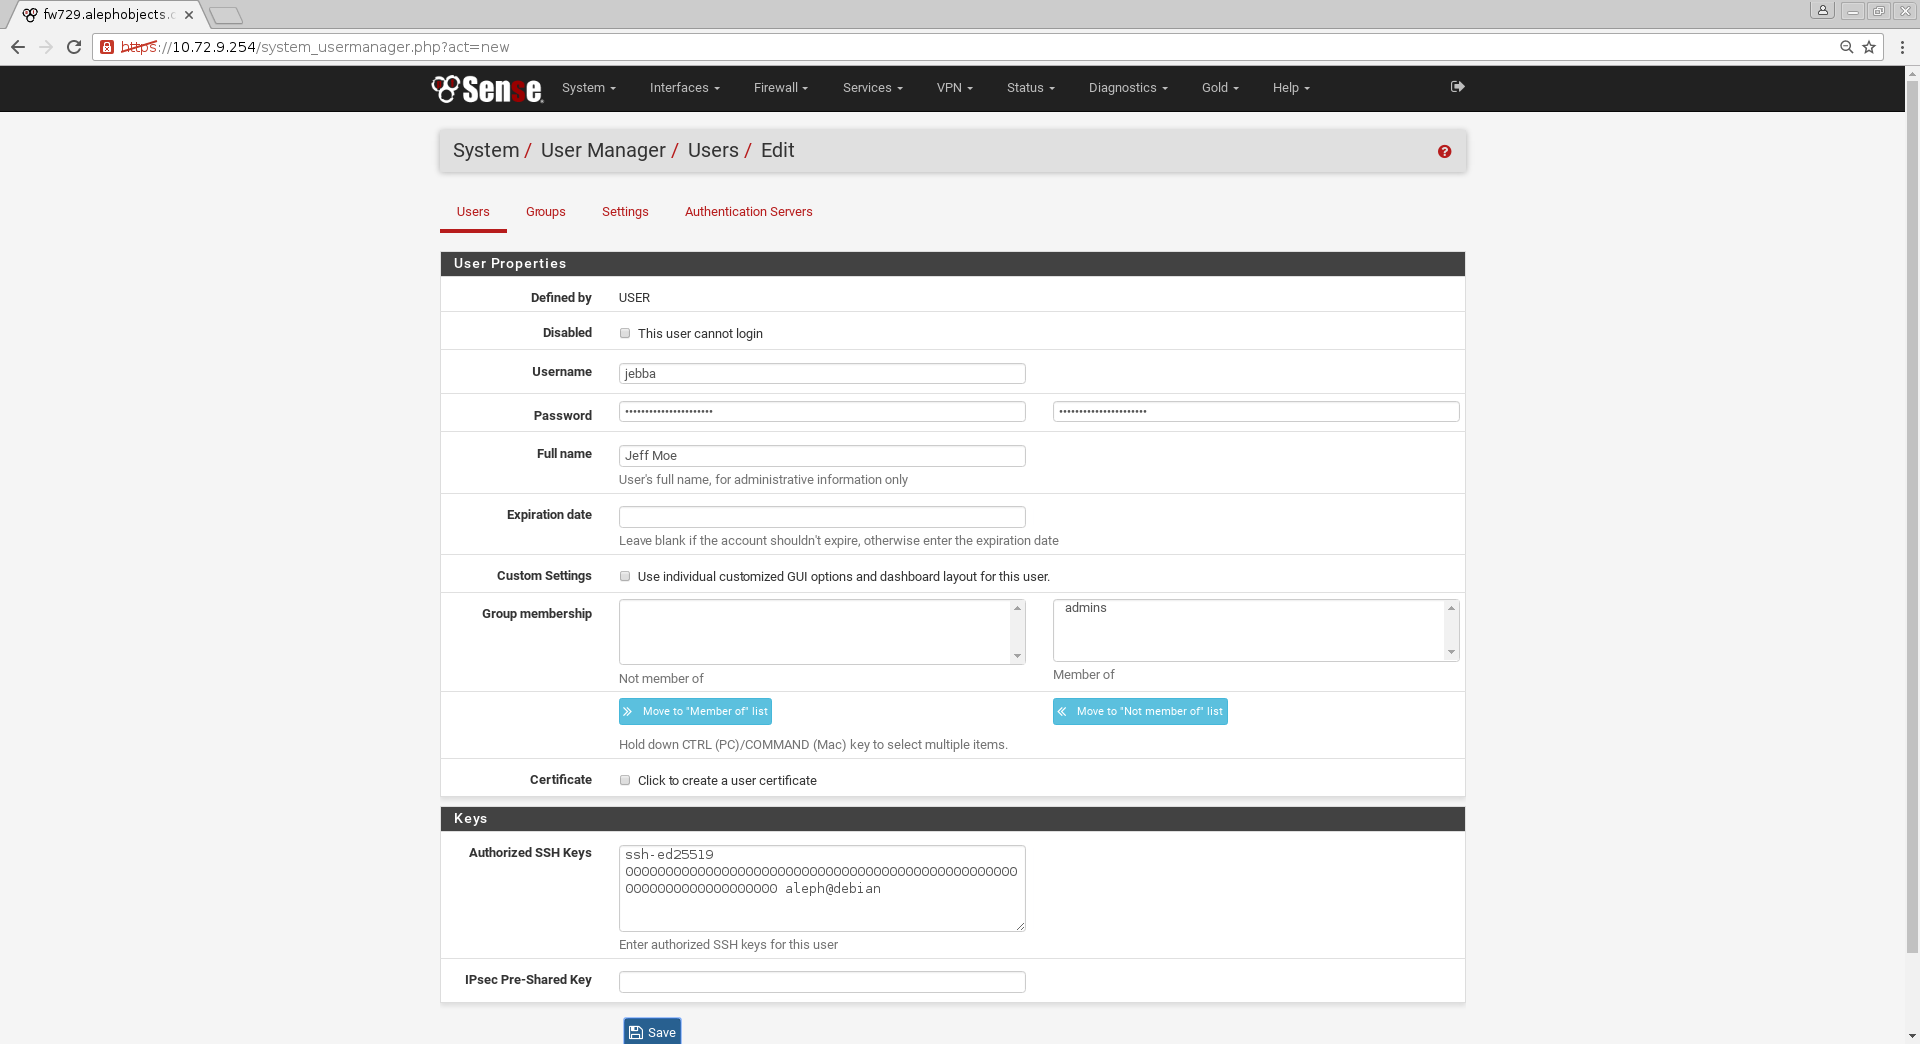
\includegraphics[keepaspectratio=true,height=0.50\textheight,width=0.75\textwidth,angle=0]{pfsense-system-user-add.png}
 \caption{pfSense Menu: System, User Manager, Add User}
 \label{fig:pfsense-system-user-add}
\end{center}
\end{figure}

 \item Add \texttt{Username}, \texttt{jebba} in this example--use something else.
 \item Add a good, well-generated unique password.
 \item Enter the user's \texttt{Full name}.
 \item \texttt{Expiration date} leave blank.
 \item Move to add to \texttt{Group membership} \texttt{admins}.
 \item \texttt{Certificate}, leave blank for now (one will be set up later with OpenVPN).
 \item For \texttt{Authorized SSH Keys}, add your SSH key from your Debian workstation. It will be either \texttt{/home/aleph/.ssh/id\_ed25519.pub} or for older keys \texttt{/home/aleph/.ssh/id\_rsa.pub}. Be sure the file ends in \texttt{.pub} and isn't the private key. You can use multiple keys, one per line.
 \item Hit \texttt{Save}.
 \item Log out as the admin user by clicking the logout icon in the upper right corner of the pfSense web page.
 \item Log back in as the newly created user and password in the above steps.
\end{enumerate}

\subsection{SSH Access}
\begin{figure}[h!]
\begin{center}
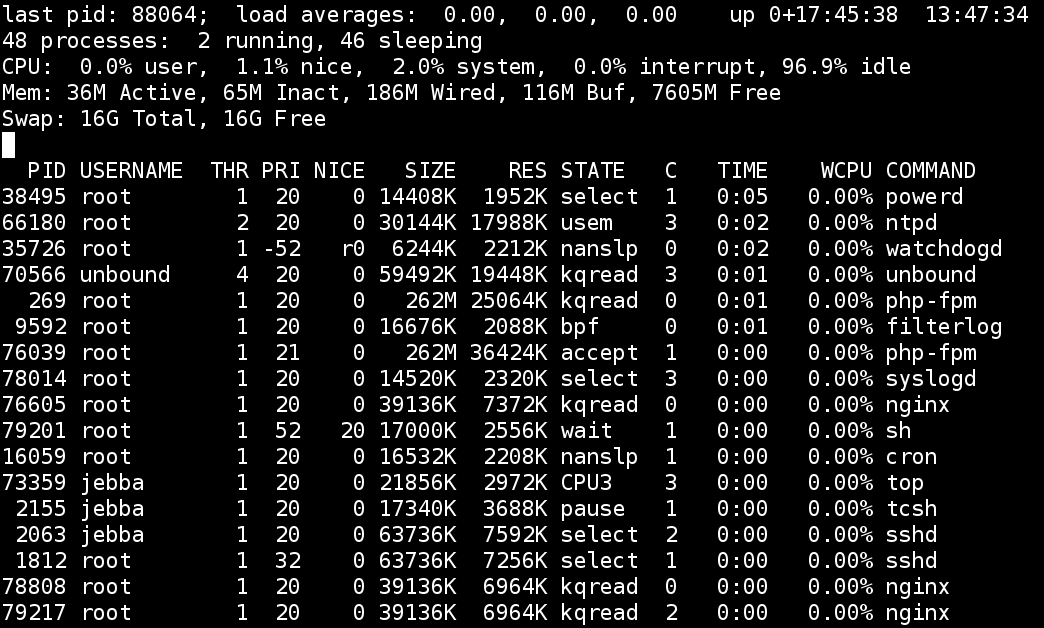
\includegraphics[keepaspectratio=true,height=0.50\textheight,width=0.75\textwidth,angle=0]{pfsense-term-top.png}
 \caption{pfSense Via SSH, Running \texttt{top}}
 \label{fig:pfsense-term-top}
\end{center}
\end{figure}
At this point, enough is set up in the router to allow for remote SSH access.
Log in, like in this example, where the port is \texttt{2222}, the user is \texttt{jebba}, and the IP address of the firewall is \texttt{10.72.9.254}.
Side note: the FreeBSD shell displays better on a black terminal than a white one.

\begin{minted}{sh}
ssh -p 2222 jebba@10.72.9.254
\end{minted}

Some example commands to run:
\begin{minted}{sh}
top # use q to exit
dmesg
df -h
ps ax
ifconfig
ping -c 1 10.72.9.254
route -n show 0.0.0.0 # Will give error if no gateway is set
# etc...
\end{minted}


\subsection{Admin Access Configuration}
\begin{figure}[h!]
\begin{center}
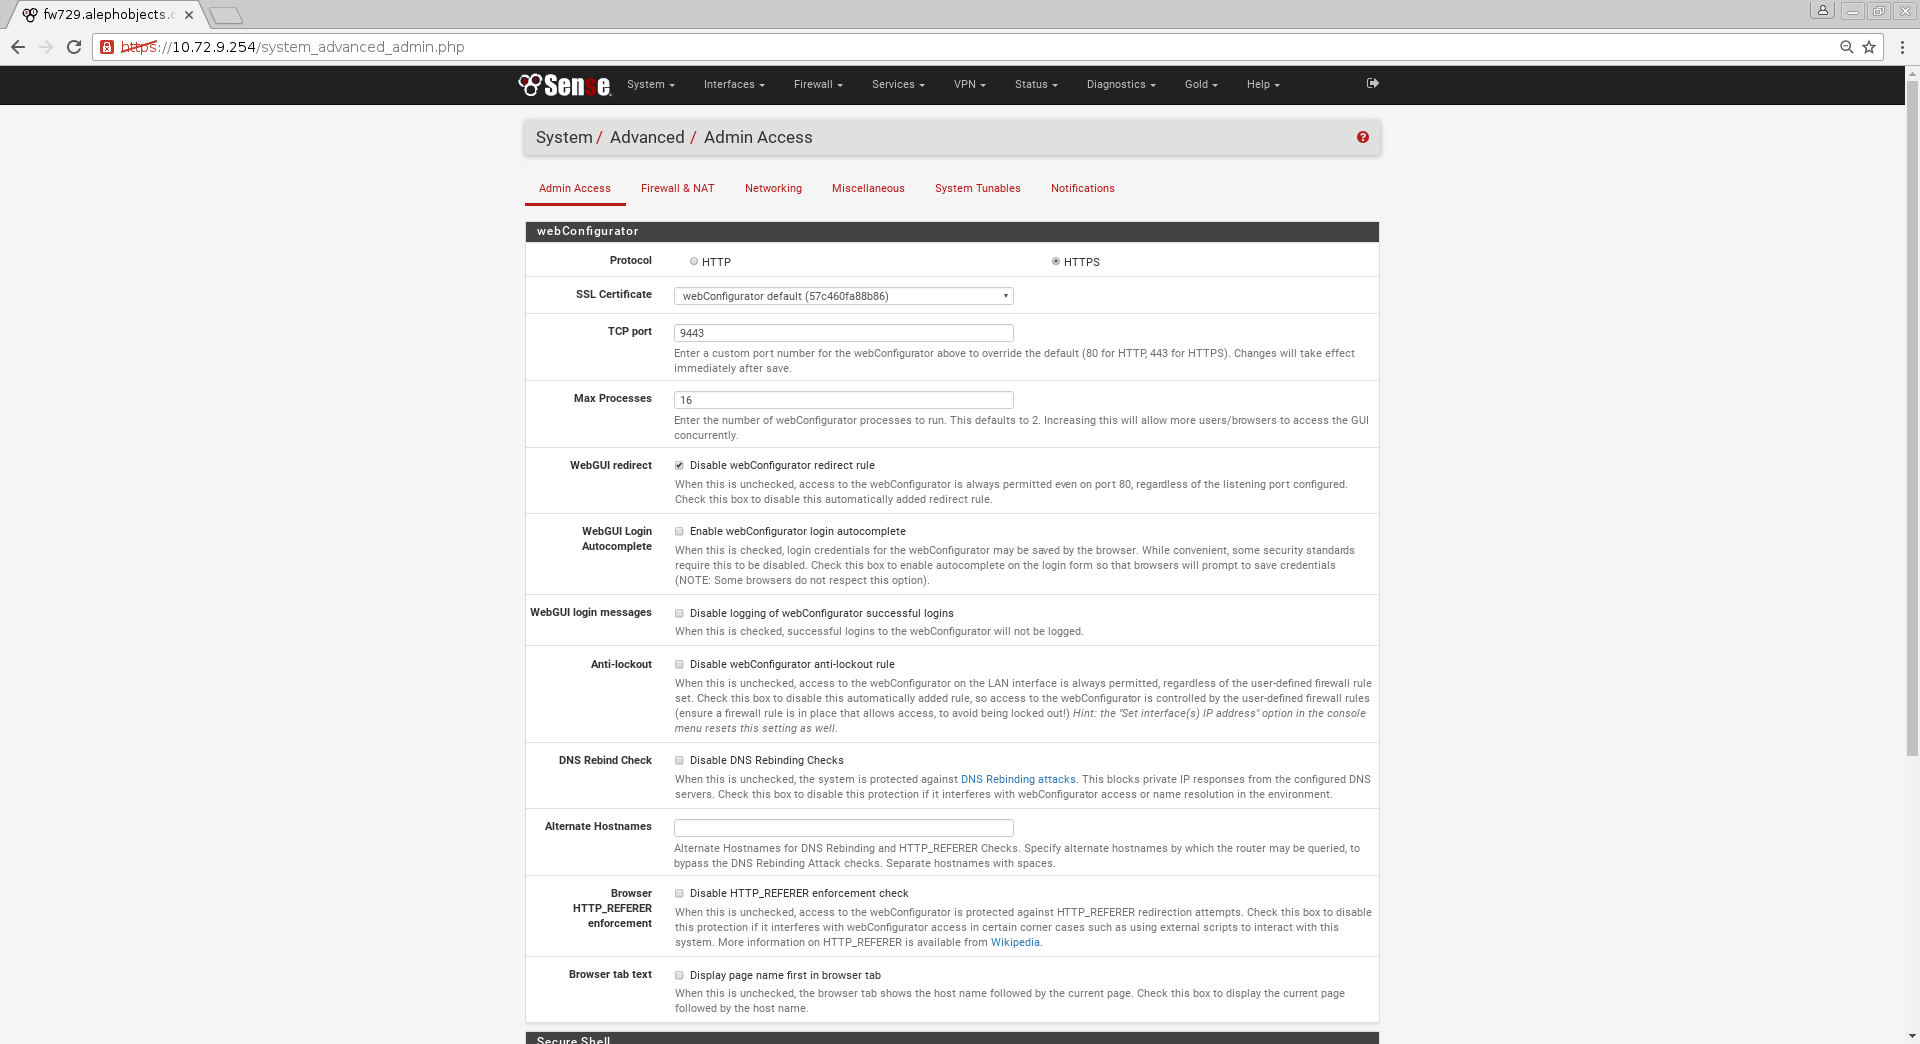
\includegraphics[keepaspectratio=true,height=0.50\textheight,width=0.75\textwidth,angle=0]{pfsense-system-adv-access.png}
 \caption{pfSense Menu: System, Advanced, Admin Access}
 \label{fig:pfsense-system-adv-access}
\end{center}
\end{figure}
\begin{enumerate}
 \item Goto \texttt{System} --> \texttt{Advanced}, \texttt{Admin Access} tab.
 \item Leave \texttt{Protocol} at \texttt{HTTPS}.
 \item Set \texttt{TCP port} to randomish port between \texttt{1} and \texttt{65535}. This will be the new pfSense web interface port address.
 \item Set \texttt{Max Processes}: 16 (2 is too low, not sure what is ideal).
 \item Check \texttt{WebGUI redirect} to disable port 80.
 
 \item Leave \texttt{WebGUI Login Autocomplete} unchecked.
 \item Leave \texttt{WebGUI login messages} unchecked.
 \item Leave \texttt{Anti-lockout} unchecked.
 \item Leave \texttt{DNS Rebind Check} unchecked.
 \item Leave \texttt{Alternate Hostnames} blank. If there are known other names for the firewall, they can be entered here.
 \item Leave \texttt{Browser HTTP\_REFERER enforcement} unchecked.
 \item Leave \texttt{Browser tab text} unchecked.
 \item Check \texttt{Secure Shell Server} to enable SSH.
 \item Check \texttt{Authentication Method} to disable password logins.
 \item Set \texttt{SSH Port} to a new randomish port btween \texttt{1} and \texttt{65535}.
 \item Leave \texttt{Serial Speed} at \texttt{115200}.
 \item Check \texttt{Console menu} to password protect the serial console menu.
 \item Hit \texttt{Save}.
 \item If a new port was set, the browser will redirect to it after a few seconds, for example to \url{https://10.72.9.254:9443/system_advanced_admin.php}
 \item At this point, you can optionally SSH into the firewall, if a key was set up for the user.
\end{enumerate}

\subsection{Advanced Networking Configuration}
Note, the \texttt{System} --> \texttt{Advanced}, \texttt{Firewall \& NAT} section can be left at defaults.

\begin{enumerate}
 \item Under \texttt{System} --> \texttt{Advanced}, \texttt{Networking} tab.
 \item Uncheck \texttt{Allow IPv6}, to disable IPv6 (yay!).
 \item Check to disable \texttt{Hardware Checksum Offloading}. This needs to be disabled for Suricata inline mode. This needs to be disabled when running pfSense inside a virtual KVM, or you'll get TCP/IP checksum errors.
 \item Check to disable \texttt{Hardware TCP Segmentation Offloading}. This needs to be disabled for Suricata inline mode.
 \item Check to disable \texttt{Hardware Large Receive Offloading}. This needs to be disabled for Suricata inline mode.
 \item Hit \texttt{Save}.
\end{enumerate}

\subsection{Advanced Miscellaneous Configuration}
\begin{enumerate}
 \item \texttt{System} --> \texttt{Advanced}, \texttt{Miscellaneous}.
 \item \texttt{Cryptographic Hardware} should be set to \texttt{AES-NI} for any hardware from pfSense. For other hardware, check dmesg.
 \item \texttt{Thermal Sensors}: use \texttt{Intel Core* CPU on-die thermal sensor}.
 \item \texttt{Hard disk standby time}, set to \texttt{6 minutes} (not sure this really has any effect).
 \item \texttt{Host UUID}, check \texttt{Do NOT send HOST UUID with user agent}.
 \item Hit \texttt{Save}.
\end{enumerate}

\subsection{Advanced Notifications Configuration}
\begin{enumerate}
 \item \texttt{System} --> \texttt{Advanced}, \texttt{Notifications}.
 \item Check to \texttt{Disable Growl Notifications}
 \item Check to \texttt{Disable SMTP}.
 \item Hit \texttt{Save}.
\end{enumerate}

\subsection{SSL Create a Certificate Signing Request}
A new SSL certificate will be created in the following steps. This certificate will then be used to
encrypt web administration sessions (\texttt{https}).

\begin{enumerate}
 \item \texttt{System} --> \texttt{Cert. Manager}, \texttt{Certificates}.
 \item Click \texttt{Add}.
 \item \texttt{Method}: \texttt{Create a Certificate Signing Request}.
 \item \texttt{Descriptive Name}, use the hostname of the firewall being setup.
 \item \texttt{Key length}: \texttt{4096}. That may be overkill, but it is just used for the CSR so it doesn't matter.
 \item \texttt{Digest Algorithm}: \texttt{sha512}.
 \item \texttt{Country Code}: \texttt{US}.
 \item \texttt{State}: \texttt{Colorado}. % XXX I think this has a different name. Region?
 \item \texttt{City}: \texttt{Loveland}.
 \item \texttt{Common name}, use hostname of firewall.
 \item Hit \texttt{Save}.
\end{enumerate}

\subsection{SSL Retrieve and Submit a Certificate Signing Request}
\begin{enumerate}
 \item \texttt{System} --> \texttt{Cert. Manager}, \texttt{Certificates}.
 \item For the new cert added above, click \texttt{Export Request} mini-icon.
 \item Go to the SSL provider, such as \url{https://gandi.net}.
 \item Gandi: \texttt{Standard SSL}, single address, 3 year.
 \item Paste in the CSR exported from the mini-icon into Gandi.
 \item Select \texttt{Apache/ModSSL} for \texttt{Software} used in Gandi, 
 \item If it says the correct \texttt{Main domain (CN)}, hit \texttt{Submit} in Gandi.
 \item Delete any temporary \texttt{*.req} file that was downloaded by browser.
 \item Gandi: \texttt{Validation by email} (probably). It will take ~10+ minutes to get verification back from Gandi (not instant).
 \item When verification email arrives, go to the URL provided and enter the provided random string.
 \item It takes around 5 minutes for the confirmation to be pushed back to Gandi and make the certificate valid. Wait.
\end{enumerate}

\subsection{SSL Install New Certificate}
\begin{enumerate}
 \item \texttt{System} --> \texttt{Cert. Manager}, \texttt{Certificates}.
 \item When cert is ready and confirmed at Gandi, hit \texttt{Get the Certificate}.
 \item Hit the \texttt{Update CSR} pencil on the appropriate certificate line.
 \item In the Gandi popup window, copy the certificate data.
 \item In the pfSense window, paste the Gandi cert into the \texttt{Final certificate data} field.
 \item Delete any downloaded copies.
\end{enumerate}

\subsection{SSL Import Gandi Certificate Authority}
Note, this has to be done after the above Gandi certificate is added to the firewall.

XXX Note, we could also import AO's key here.

\begin{enumerate}
 \item \texttt{System} --> \texttt{Cert. Manager}, \texttt{CAs}.
 \item Under \texttt{CAs}, click \texttt{Add}.
 \item \texttt{Method}: \texttt{Import an existing Certificate Authority}.
 \item \texttt{Descriptive Name}: \texttt{GandiStandardSSLCA2}.
 \item Download the cert from \url{https://www.gandi.net/static/CAs/GandiStandardSSLCA2.pem}
 \item Paste downloaded Gandi certificate into \texttt{Certificate data}.
 \item Leave \texttt{Certificate Private Key} blank.
 \item Hit \texttt{Save}.
\end{enumerate}

\subsection{SSL Certificate Revocations}
Note, this has to be done after the above Gandi certificate is added to the firewall.

\begin{enumerate}
 \item \texttt{System} --> \texttt{Cert. Manager}, \texttt{Certificate Revocations}.
 \item Import \texttt{Certificate Revocations}, if any.
\end{enumerate}

\subsection{General Setup}
\begin{enumerate}
 \item \texttt{System} --> \texttt{General Setup}.
 \item Leave most at defaults.
 \item \texttt{Top Navigation}: \texttt{Fixed (Remains visible at top of page)}.
 \item \texttt{Hostname in Menu}: \texttt{Hostname only}.
 \item \texttt{DNS servers} can be bound to particular interfaces here, if needed in multi-WAN (later configuration).
 \item \texttt{Dashboard Columns} set to \texttt{4}.
 \item Hit \texttt{Save}.
\end{enumerate}

\subsection{Use New SSL Certificate for Web Admin}
A new SSL certificate was created above. This can now be used by the firewall to encrypt web administration sessions.

\begin{enumerate}
 \item \texttt{System} --> \texttt{Advanced}, \texttt{Admin Access}.
 \item Change \texttt{SSL Certificate} to the new one created above.
 \item Hit \texttt{Save}.
 \item Now go to that new hostname with https and the correct port, such as \url{https://10.72.9.254:9443/}.
\end{enumerate}

\subsection{Initial Firewall Rules}
Some basic firewall rules will be set up now, before the WAN interface is enabled.
For now, IPv6 will be rejected on the LAN interface and blocked on the WAN interface.

\begin{enumerate}
 \item \texttt{Firewall} --> \texttt{Rules}, \texttt{LAN}.
 \item \texttt{LAN} interface, click the pencil to edit the \texttt{IPv6} line.
 \item Change \texttt{Action} to \texttt{Reject}.
 \item Change \texttt{Source} to \texttt{any}.
 \item Change \texttt{Description} to \texttt{Default Reject LAN IPv6}.
 \item Hit \texttt{Save}.
 \item Hit \texttt{Apply Changes}.
 \item \texttt{Firewall} --> \texttt{Rules}, \texttt{LAN}.
 \item Click the \texttt{Copy} mini-icon to copy the newly modified \texttt{IPv6} line.
 \item Change \texttt{Action} to \texttt{Block}.
 \item Change \texttt{Interface} to \texttt{WAN}.
 \item Change \texttt{Description} to \texttt{Default Block WAN IPv6}.
 \item Hit \texttt{Save}.
 \item Hit \texttt{Apply Changes}.
\end{enumerate}

\subsection{Initial DNS Resolver Setup}
\begin{enumerate}
 \item \texttt{Services} --> \texttt{DNS Resolver}.
 \item Check \texttt{Enable} (default).
 \item \texttt{Network Interfaces}: select \texttt{LAN} and \texttt{localhost}.
 \item \texttt{Outgoing Network Interfaces}: select \texttt{WAN}, \texttt{LAN}, \texttt{localhost}.
 \item Check \texttt{DHCP Registration}
 \item Check \texttt{Static DHCP}
 \item Hit \texttt{Save}.
 \item Hit \texttt{Apply Changes}.
 \item \texttt{Services} --> \texttt{DNS Resolver}, \texttt{Advanced Settings}.
 \item Check \texttt{Prefetch Support}.
 \item Check \texttt{Prefetch DNS Key Support}.
 \item Increase \texttt{Message Cache Size} to \texttt{50 MB} or so (?).
 \item Hit \texttt{Save}.
 \item Hit \texttt{Apply Changes}.
\end{enumerate}

\subsection{Dynamic DNS Setup}
If dynamic DNS is to be set up, follow these steps... XXX
\begin{enumerate}
 \item \texttt{Services} --> \texttt{Dynamic DNS}.
\end{enumerate}

\subsection{Initial Logging Setup}
Setup logging to the local firewall. Remote logging will be set up.

\begin{enumerate}
 \item \texttt{Status} --> \texttt{System Logs}, \texttt{Settings}.
 \item Check \texttt{Forward/Reverse Display}.
 \item Increase \texttt{GUI Log Entries} to \texttt{200}.
 \item Set \texttt{Where to show rule descriptions} to \texttt{Display as second row}.
 \item Note, XXX this is where remote logging will be set up... 
 \item Hit \texttt{Save}.
\end{enumerate}

\subsection{Initial Dashboard Setup}

\begin{enumerate}
 \item \texttt{Status} --> \texttt{Dashboard}.
 \item Click the Plus \texttt{+} in the upper right corner.
 \item Add \texttt{Firewall Logs}.
 \item Add \texttt{Gateways}.
 \item Add \texttt{Interface Statistics}.
 \item Add \texttt{NTP Status}.
 \item Add \texttt{OpenVPN}.
 \item Add \texttt{Services Status}.
 \item Add \texttt{S.M.A.R.T. Status}.
 \item Add \texttt{Thermal Sensors}.
 \item Add \texttt{Traffic Graphs}.
 \item Click the mini-disk icon in the upper right to save the dashboard configuration.
\end{enumerate}

\subsection{Backup}
Make first backup.

\begin{enumerate}
 \item \texttt{Diagnostics} --> \texttt{Backup \& Restore}, \texttt{Backup}.
 \item Make a backup and store in the proper location.
\end{enumerate}

\subsection{Reboot}
Now that most of the ``initial'' setup has been done, reboot to make sure everything comes up clean.
It takes less than two minutes to reboot. XXX times.

\begin{enumerate}
 \item \texttt{Diagnostics} --> \texttt{Reboot}
\end{enumerate}

\subsection{Internet Connection}
Make initial connection to the Internet with the new pfSense firewall.


At this point, this presumes the WAN interface isn't up and routing actual Internet traffic. It is better to get the router as configured as possible before actually using the WAN interface. Assuming the firewall is on the LAN and being configured, it can use the gateway that is on its LAN interface. When configuration is finalized and the router is deployed, the WAN interface will carry Internet traffic. To to this, add a route by: Interfaces --> LAN. Under IPv4 Upstream gateway, click Add a new gateway. Add the LAN gateway info, and check is as Default gateway (3000). Save. Apply Changes..

\begin{enumerate}
 \item \texttt{System} --> \texttt{Routing}
 \item Click to \texttt{Edit} the mini pencil icon on the \texttt{Gateway} line listed as \texttt{Default}.
 \item \texttt{Monitor IP}: something appropriate upstream, can use \texttt{8.8.8.8}.
 \item Note: on high latency connections such as satellite, hit \texttt{Display Advanced} and increase \texttt{Latency thresholds} (default: 750, new: 2500), \texttt{Packet Loss thresholds} (15, 25), \texttt{Probe Interval} (1000), \texttt{Loss Interval} (3000).
 \item Hit \texttt{Save}.
 \item Hit \texttt{Apply Changes}.
\end{enumerate}

\subsection{Update \& Install Packages}
\begin{enumerate}
 \item \texttt{System} --> \texttt{Update}, \texttt{System Update}.
 \item Check that the \texttt{Status} is \texttt{Up to date}. If it needs updating, hit \texttt{Update}.
 \item \texttt{System} --> \texttt{Package Manager}, \texttt{Installed Packages}.
 \item The first time here, you need to click on \texttt{Available Packages}
 \item Wait to download latest package header info.
 \item Then go back to \texttt{System} --> \texttt{Package Manager}, \texttt{Installed Packages}.
 \item If there are any \texttt{Installed Packages} that have a \texttt{Newer version available}, click the mini icon to \texttt{Update} the package. Then \texttt{Confirm}.
 \item Go to \texttt{System} --> \texttt{Package Manager}, \texttt{Available Packages} and install the following packages:
 \item \texttt{Cron}.
 \item \texttt{ntopng}.
 \item \texttt{openvpn-client-export}.
 \item \texttt{pfBlockerNG}.
 \item \texttt{RRD\_Summary}.
 \item \texttt{Status\_Traffic\_Totals}.
 \item \texttt{sudo}.
 \item \texttt{suricata}.
\end{enumerate}

\subsection{Set Up \texttt{sudo} User}
\begin{enumerate}
 \item \texttt{System} --> \texttt{sudo}
 \item Add the user added above to sudo.
\end{enumerate}

\subsection{OpenVPN Certificates}
OpenVPN certificates need to be created before OpenVPN can be set up.
Also, new DH random seeds are generated.

\begin{enumerate}
 \item SSH into firewall. pfSense ships with pre-generated DH keys, due to ``heavy computation''. This can take an hour for 4096.
\begin{minted}{sh}
/usr/bin/openssl dhparam 1024 > /etc/dh-parameters.1024
/usr/bin/openssl dhparam 2048 > /etc/dh-parameters.2048
/usr/bin/openssl dhparam 4096 > /etc/dh-parameters.4096
\end{minted}
 \item System --> Cert. Manager. Set up internal certificate authority. XXX Add Steps
 \item System --> Cert. Manager. Create internal server certificate. XXX Add steps
\end{enumerate}

\subsection{OpenVPN Setup}
\begin{enumerate}
 \item \texttt{VPN} --> \texttt{OpenVPN}
 \item Set up VPN server.
 \item \texttt{Server Mode}: \texttt{Remote Access (SSL/TLS + User Auth)}.
 \item \texttt{Backend for Authentication}: \texttt{Local Database} (will be FreeRADIUS at some point).
 \item \texttt{Protocol}: \texttt{UDP}.
 \item \texttt{Local Port}: something randomish. Note for later.
 \item \texttt{Peer Certificate Authority}: use the interal CA created earlier.
 \item \texttt{Server Certificate}: Use the server certificate created earlier.
 \item \texttt{DH Parameter length (bits)}: \texttt{4096}.
 \item \texttt{Encryption Algorithm}: \texttt{AES-256-CBC (256-bit)}. This algorithm has hardware crypto support on pfSense routers. In pfSense 2.4, \texttt{AES-256-GCM} may be supported and is preferred.
 \item \texttt{Auth digest algorithm}: \texttt{SHA512 (512-bit)}.
 \item \texttt{Hardware Crypto}: \texttt{BSD Cryptodev engine- RSA, DSA, DH, AES-128-CBC, AES-192-CBC, AES-256-CBC}.
 \item \texttt{Certificate Depth}: \texttt{One}.
 \item \texttt{Strict User-CN Matching}: check \texttt{Enforce Match} once VPN is confirmed working. Leave unchecked for now.
 \item \texttt{IPv4 Tunnel Network}: Set the new VPN network.
 \item \texttt{IPv6 Tunnel Network}: leave blank.
 \item \texttt{Redirect Gateway}: unchecked.
 \item \texttt{IPv4 Local network(s)}: set the local LAN network, in this case \texttt{10.72.9.0/24}.
 \item \texttt{IPv6 Local network(s)}: leave blank.
 \item \texttt{Compression}: \texttt{Enabled with Adaptive Compression}.
 \item \texttt{Inter-client communication}: Checked.
 \item \texttt{Disable IPv6}: Checked.
 \item \texttt{Dynamic IP}: Unchecked, at least for now.
 \item \texttt{Topology}: \texttt{subnet}.
 \item \texttt{DNS Default Domain}: Checked, and set domain.
 \item \texttt{DNS Server enable}: Checked.
 \item \texttt{DNS Server 1}: enter servers.
 \item Hit \texttt{Save}.
\end{enumerate}

\subsection{OpenVPN User Certificate Creation}
Each user needs their own certificate, which can be tied to their user account on the firewall. Note, FreeRADIUS will be used for user authentication in the future.

XXX this needs to be checked.

\begin{enumerate}
 \item \texttt{System} --> \texttt{User Manager}
 \item Click \texttt{Add}, to create a new VPN user.
 \item \texttt{Certificate}: Check to create user certificate.
 \item \texttt{Descriptive name}: enter a \texttt{username.domainname}, such as \texttt{jebbavpn.alephobjects.com}.
 \item \texttt{Certificate Authority}: Select internal CA created above.
 \item \texttt{Key length}: \texttt{2048}.
 \item \texttt{Lifetime}: \texttt{1095}.
 \item Hit \texttt{Save}.
\end{enumerate}

\subsection{OpenVPN User Certificate Export}
Each user needs their own certificate, which can be tied to their user account on the firewall. Note, FreeRADIUS will be used for user authentication in the future.

XXX this needs to be checked.

\begin{enumerate}
 \item \texttt{VPN} --> \texttt{OpenVPN}, \texttt{Client Export}
 \item \texttt{Remote Access Server}: Select the VPN server created earlier.
 \item \texttt{Verify Server CN}: \texttt{automatic}.
 \item \texttt{Block Outside DNS}: Checked.
 \item At the bottom, export as \texttt{Standard Configurations}, \texttt{Archive} to use with another pfSense server (XXX correct?).
 \item To use with OpenVPN in F-Droid (Android), use \texttt{Inline Configurations (Android)}.
\end{enumerate}


\subsection{Turn off Internet via LAN}
If the WAN gateway has been set up, disable the LAN gateway.

\begin{enumerate}
 \item \texttt{Interfaces} --> \texttt{LAN}
 \item Change \texttt{IPv4 Upstream gateway} to \texttt{None}.
 \item Hit \texttt{Save}.
 \item Hit \texttt{Apply Changes}.
\end{enumerate}

\subsection{Backup}
Make another backup.

\begin{enumerate}
 \item \texttt{Diagnostics} --> \texttt{Backup \& Restore}, \texttt{Backup}.
 \item Make a backup and store in the proper location.
\end{enumerate}

\subsection{Reboot}
Reboot to make sure everything comes up clean.

\begin{enumerate}
 \item \texttt{Diagnostics} --> \texttt{Reboot}
\end{enumerate}

\section{NAT}
Network Address Translation.

\begin{itemize}
 \item VoIP using SIP is often a problem behind a NAT.
 \item Enable Keepalives in Grandstream phones to connect to the Asterisk server.
 \item Disable ALG (Application Level Gateway) in any consumer/home routers.
\end{itemize}


\section{Traffic Shaping}
\begin{itemize}
 \item Prioritize admin ssh to firewalls/servers (in case of DoS, etc.)
 \item Prioritize VoIP
 \item De-prioritize SMTP, etc...
\end{itemize}

\section{pfBlockerNG}
\begin{itemize}
 \item IP blocklists for botnets, etc.
\end{itemize}


\section{Suricata}
Suricata is being used as an Intrusion Detection System.
It is preferred over Snort as Suricata is multithreaded and Snort isn't.

\begin{figure}[h!]
\begin{center}
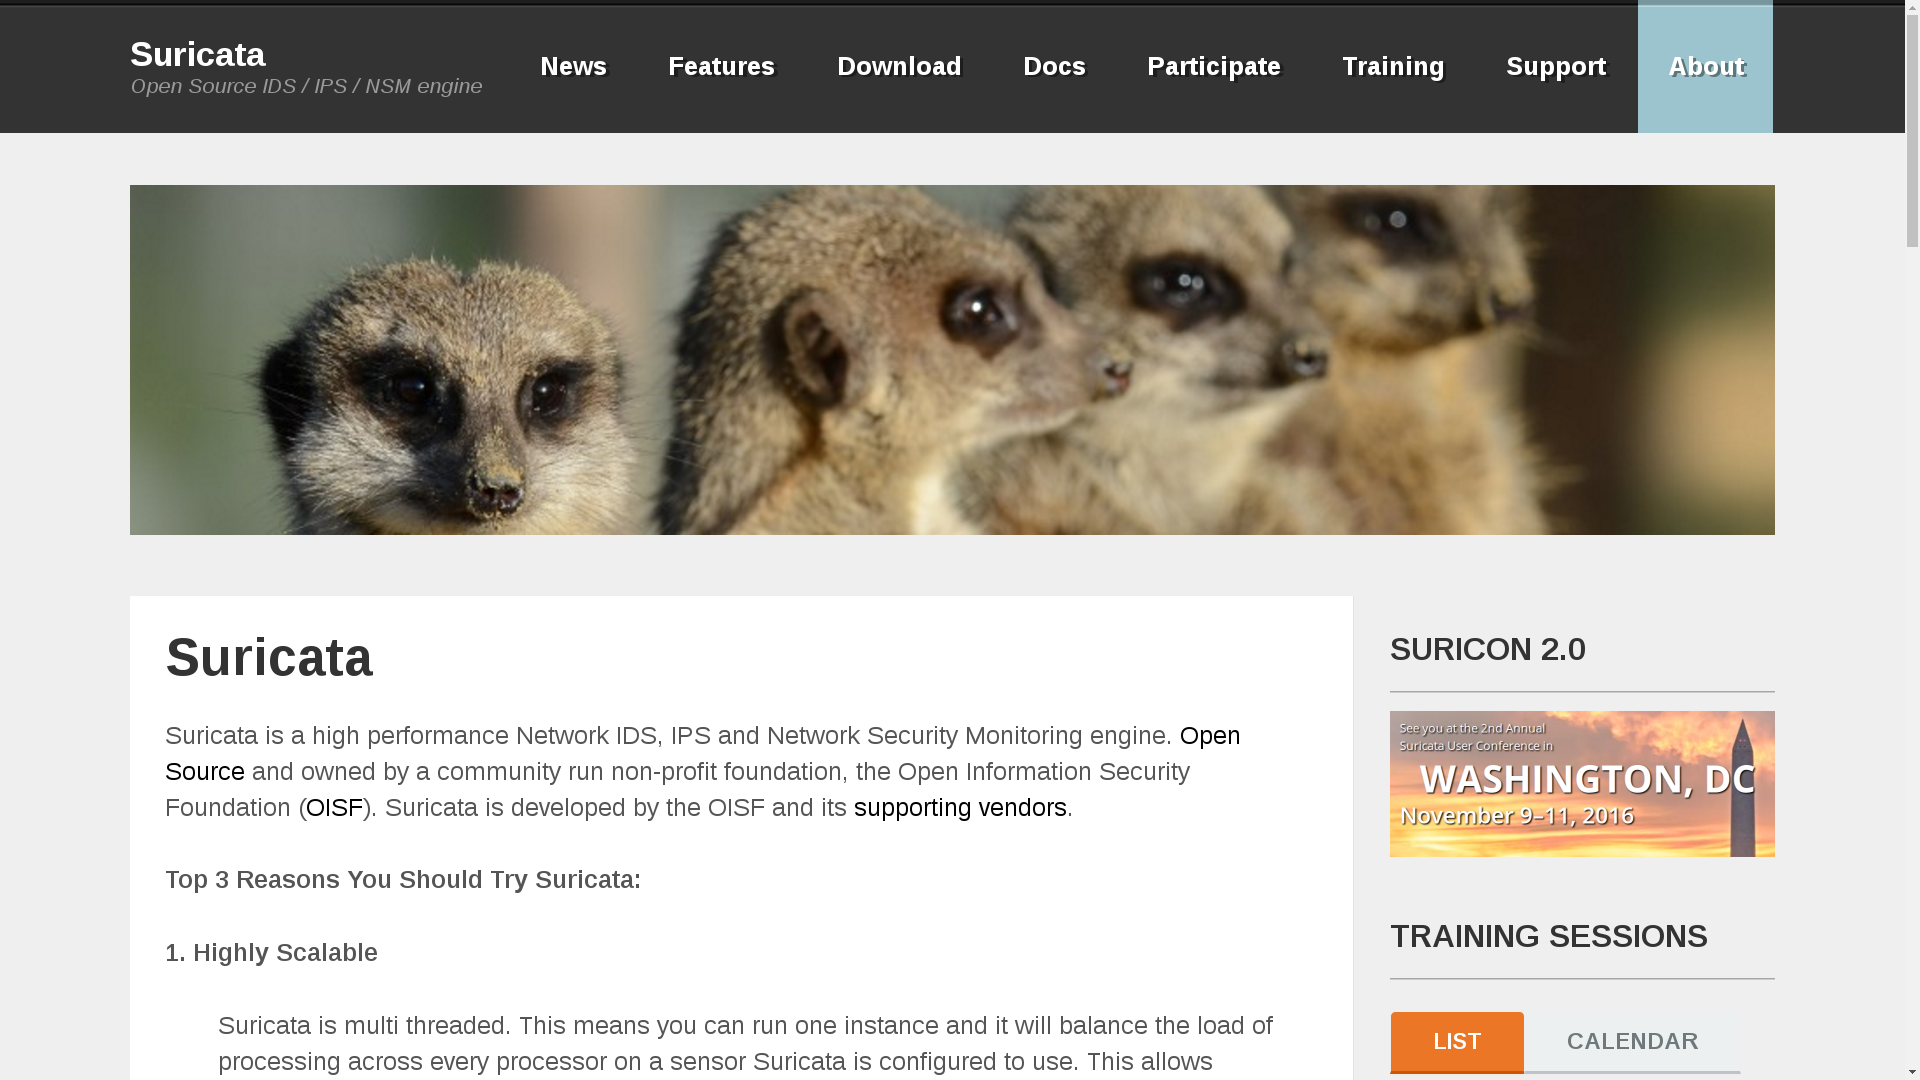
\includegraphics[keepaspectratio=true,height=0.50\textheight,width=0.75\textwidth,angle=0]{www-suricata.png}
 \caption{Suricata Website}
 \label{fig:www-suricata}
\end{center}
\end{figure}

\begin{itemize}
 \item barnyard2
 \item Snort Blacklists
 \item Emerging Threats Blacklists
 \item GeoIP
 \item Alerts, Blocks, Suppress
 \item SID
\end{itemize}


\section{DHCP}
For DHCP services, pfSense uses Dnsmasq, which is also used for DNS
forwarding.


%Services --> DHCP Server. Note: for netboot install of a workstation. Set up DHCP address. Network Booting, show advanced. Enable network booting for that host. Set Next Server to the IP address of the tftp server. Set XXX to ``jessie_crypto'' for encrypted install or ``jessie'' for a regular install.
\begin{enumerate}
 \item Services --> DHCP Server. Network Booting, click Display Advanced. Check box for Enables Network Booting. Set Default BIOS file name to jessie\_crypto/pxelinux.0 or jessie/pxelinux.0. Set Next Server to IP address of tftp server. Save.
 \item Services --> DHCP Server. Go to the bottom and hit Add. Add the MAC address, Client Identifier (hostname), IP Address, Hostname, Netboot Filename (we probably don't need it in the general config), and TFTP Server.
\end{enumerate}

\begin{itemize}
 \item Disable IPv6.
 \item tftp netboot installs.
 \item Static mappings.
\end{itemize}


\section{NTP}


\section{OpenVPN}
\begin{figure}[h!]
\begin{center}
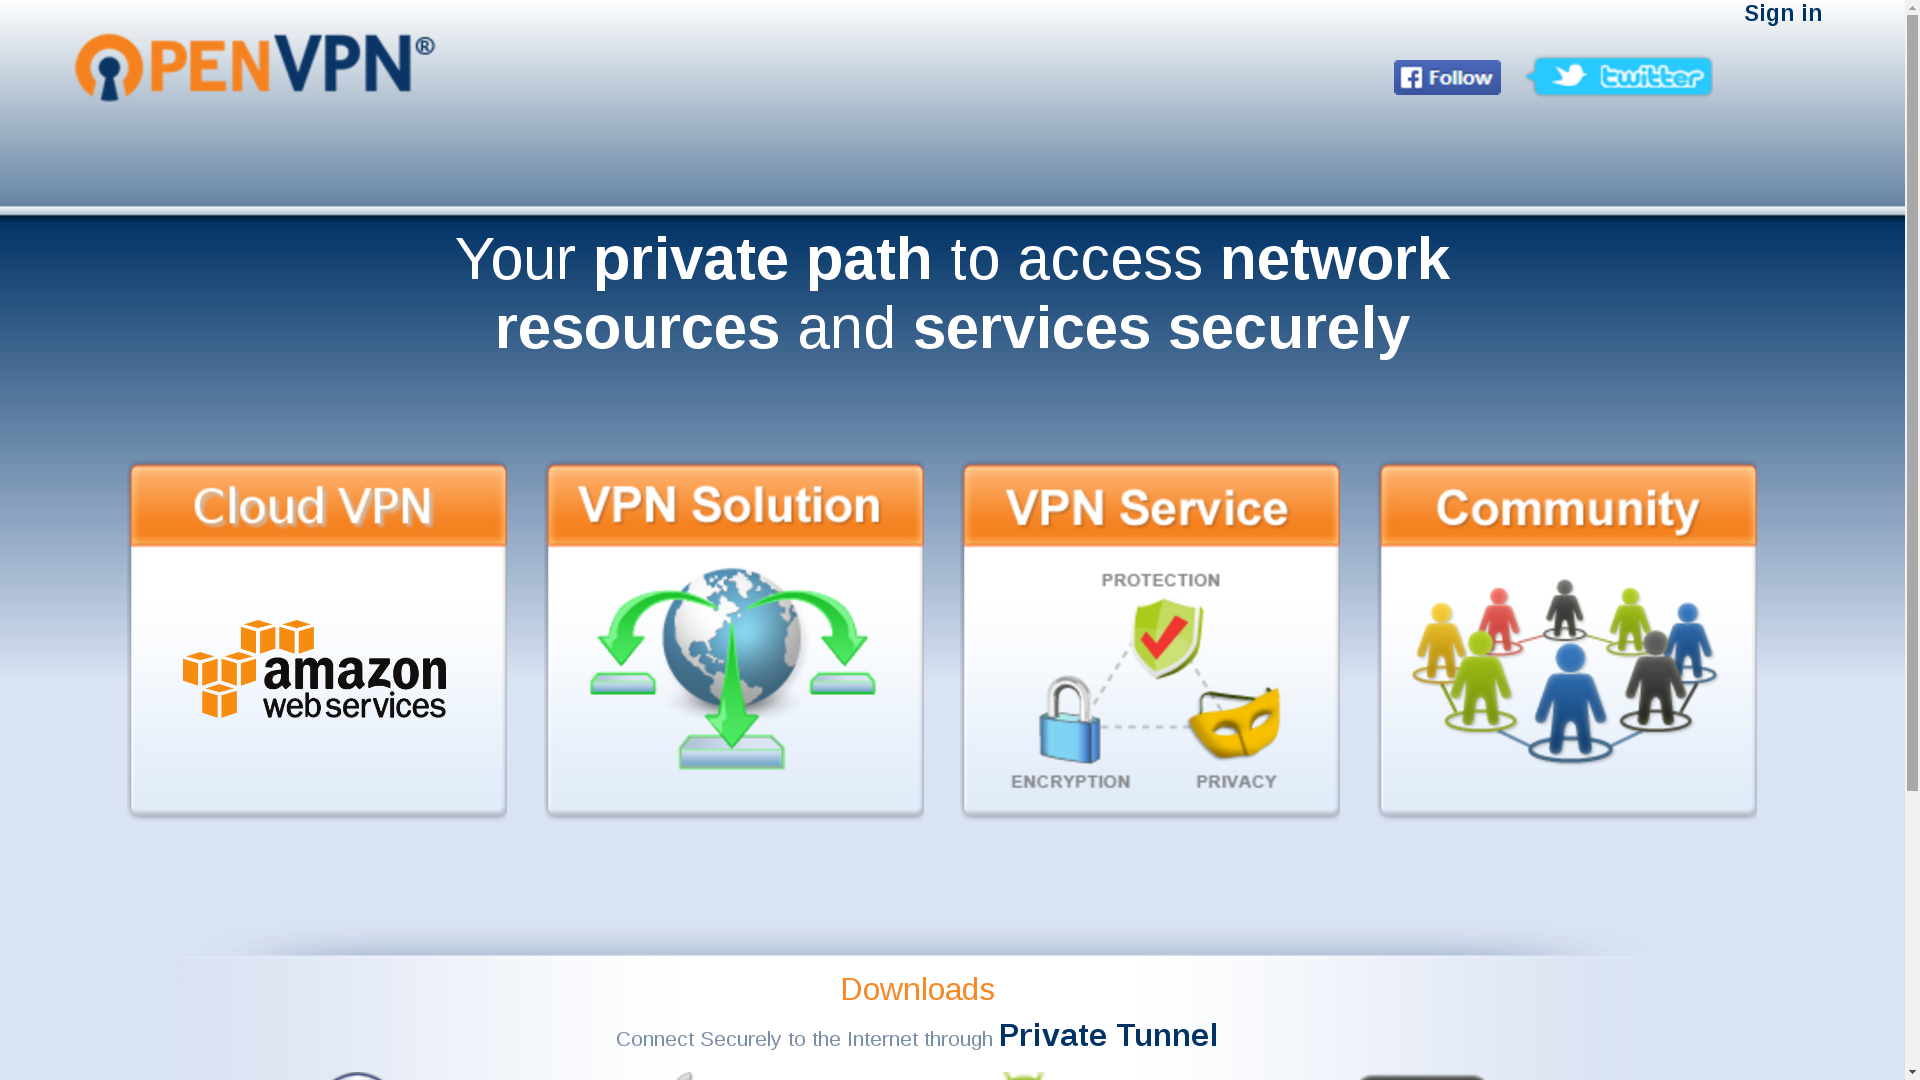
\includegraphics[keepaspectratio=true,height=0.50\textheight,width=0.75\textwidth,angle=0]{www-openvpn.png}
 \caption{OpenVPN Website}
 \label{fig:www-openvpn}
\end{center}
\end{figure}


Virtual Private Networks.


\href{https://www.openvpn.net/}{OpenVPN} --- ``OpenVPN is a full-featured open source SSL VPN solution that accommodates a wide range of configurations, including remote access, site-to-site VPNs, Wi-Fi security, and enterprise-scale remote access solutions with load balancing, failover, and fine-grained access-controls.''

\begin{itemize}
 \item Network design (e.g. many point to point, one central server, etc.).
 \item Main OpenVPN server.
 \item Other internal servers.
 \item External servers private connections.
 \item Laptops.
 \item Mobiles.
 \item SSL certificates.
 \item AES-256-CBC is hardware accelerated on pfSense routers.
 \item SHA512 Auth digest algorithm
 \item Hardware Crypto: BSD cryptodev engine
\end{itemize}


pfSense ships with pre-generated DH keys, due to ``heavy computation''.
This can take an hour for 4096.
\begin{minted}{sh}
/usr/bin/openssl dhparam 1024 > /etc/dh-parameters.1024
/usr/bin/openssl dhparam 2048 > /etc/dh-parameters.2048
/usr/bin/openssl dhparam 4096 > /etc/dh-parameters.4096
\end{minted}



\section{Captive Portal}
The Captive Portal for Aleph Mountain building wifi services.


\section{SSL Certificates}
pfSense makes it very easy to generate Certificate Signing Requests (CSRs),
which can be send to Gandi.net to get issued a ``properly'' signed SSL
certificate.


\section{ssh}
OpenSSH from OpenBSD is used. The BSD shell is a bit different from GNU.


\section{DNS}
DNS forwarding is provided by Dnsmasq.

\begin{figure}[h!]
\begin{center}
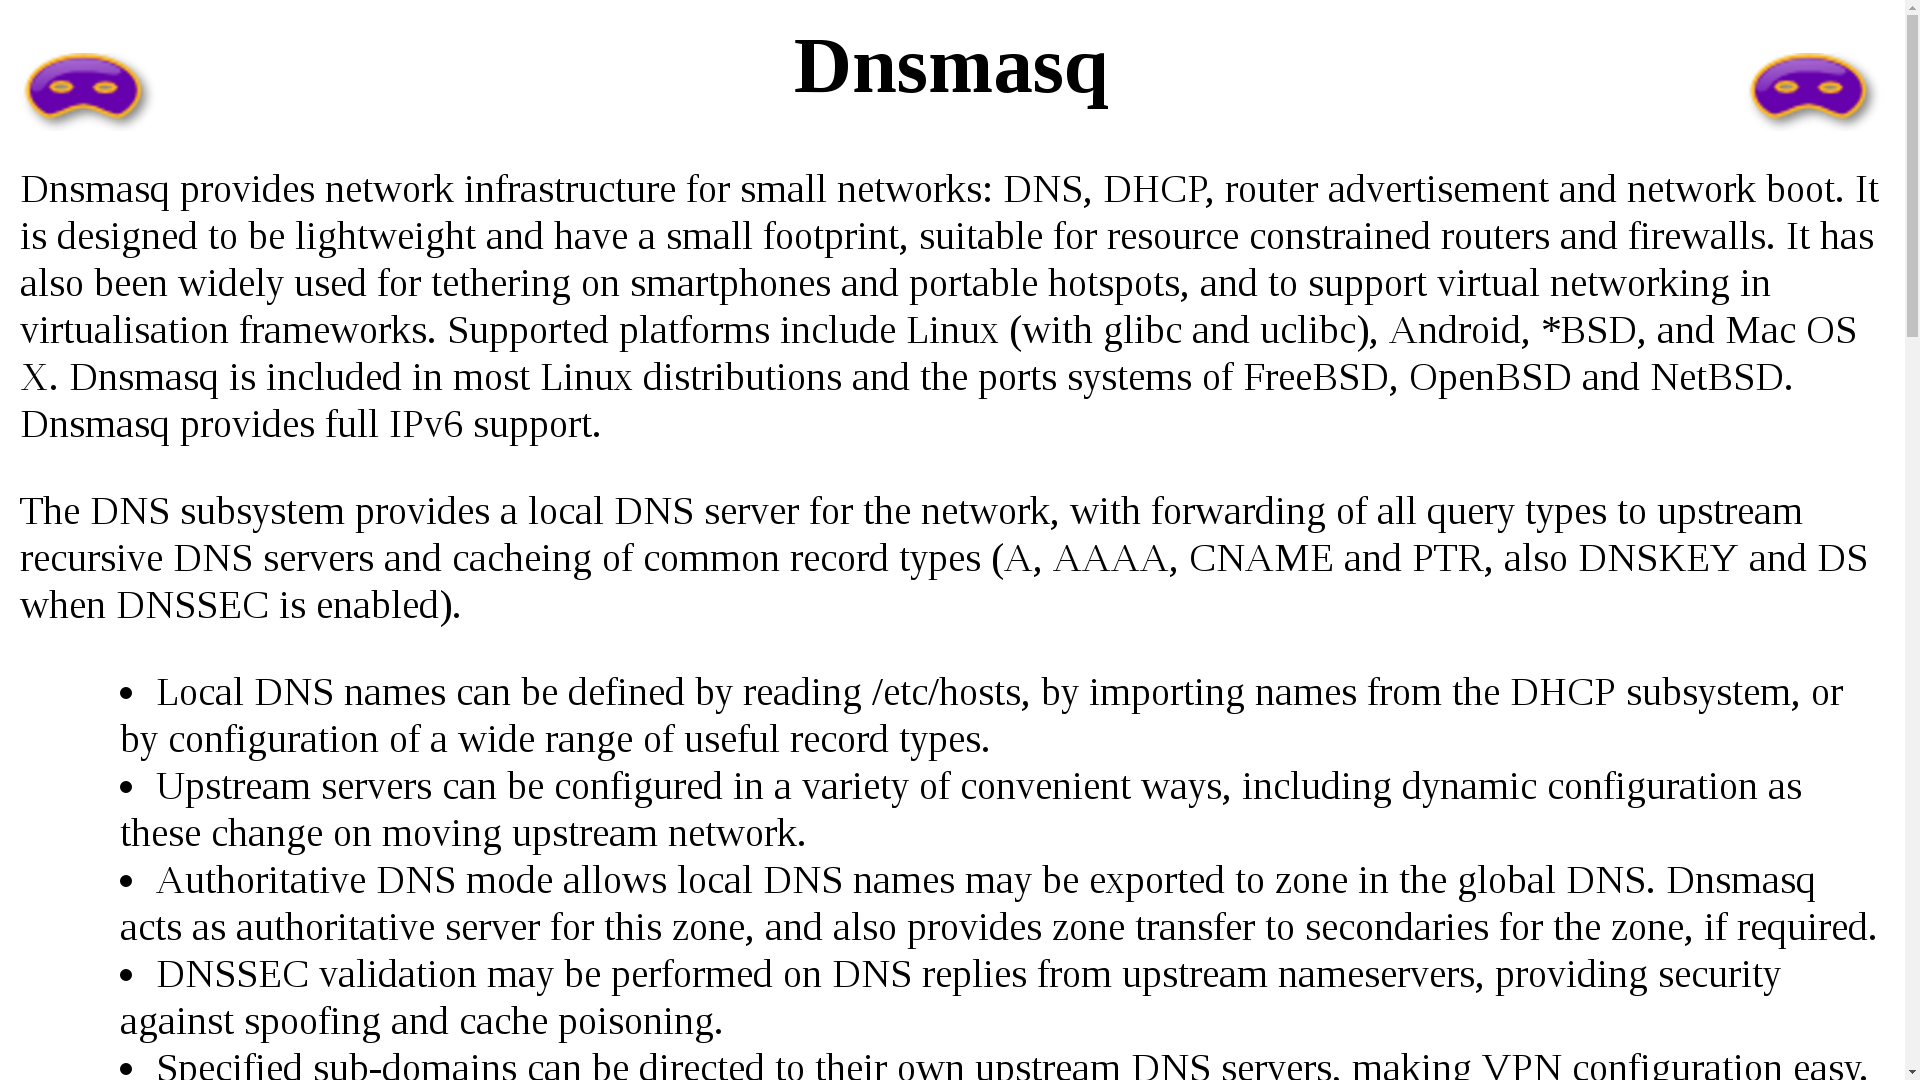
\includegraphics[keepaspectratio=true,height=0.50\textheight,width=0.75\textwidth,angle=0]{www-dnsmasq.png}
 \caption{Dnsmasq Website}
 \label{fig:www-dnsmasq}
\end{center}
\end{figure}



\section{Routing}
\begin{itemize}
 \item No BGP, OSPF, etc.
 \item Static backbone routes.
 \item WAN failover
\end{itemize}


\section{Interfaces}

\begin{itemize}
 \item Gigabit ethernet.
 \item SFP+.
 \item Hardware offloading (e.g. checksums).
\end{itemize}


\section{CARP and Synchronization}
CARP can be used to have transparent failover to another firewall, if one
firewall on the network should drop.

Synchronization between CARP firewalls allows easy configuration updates. For
instance, if a configuration change is made to the DHCP server, it can
``instantly'' push to the backup firewall.


\section{Reporting}

\begin{figure}[h!]
\begin{center}
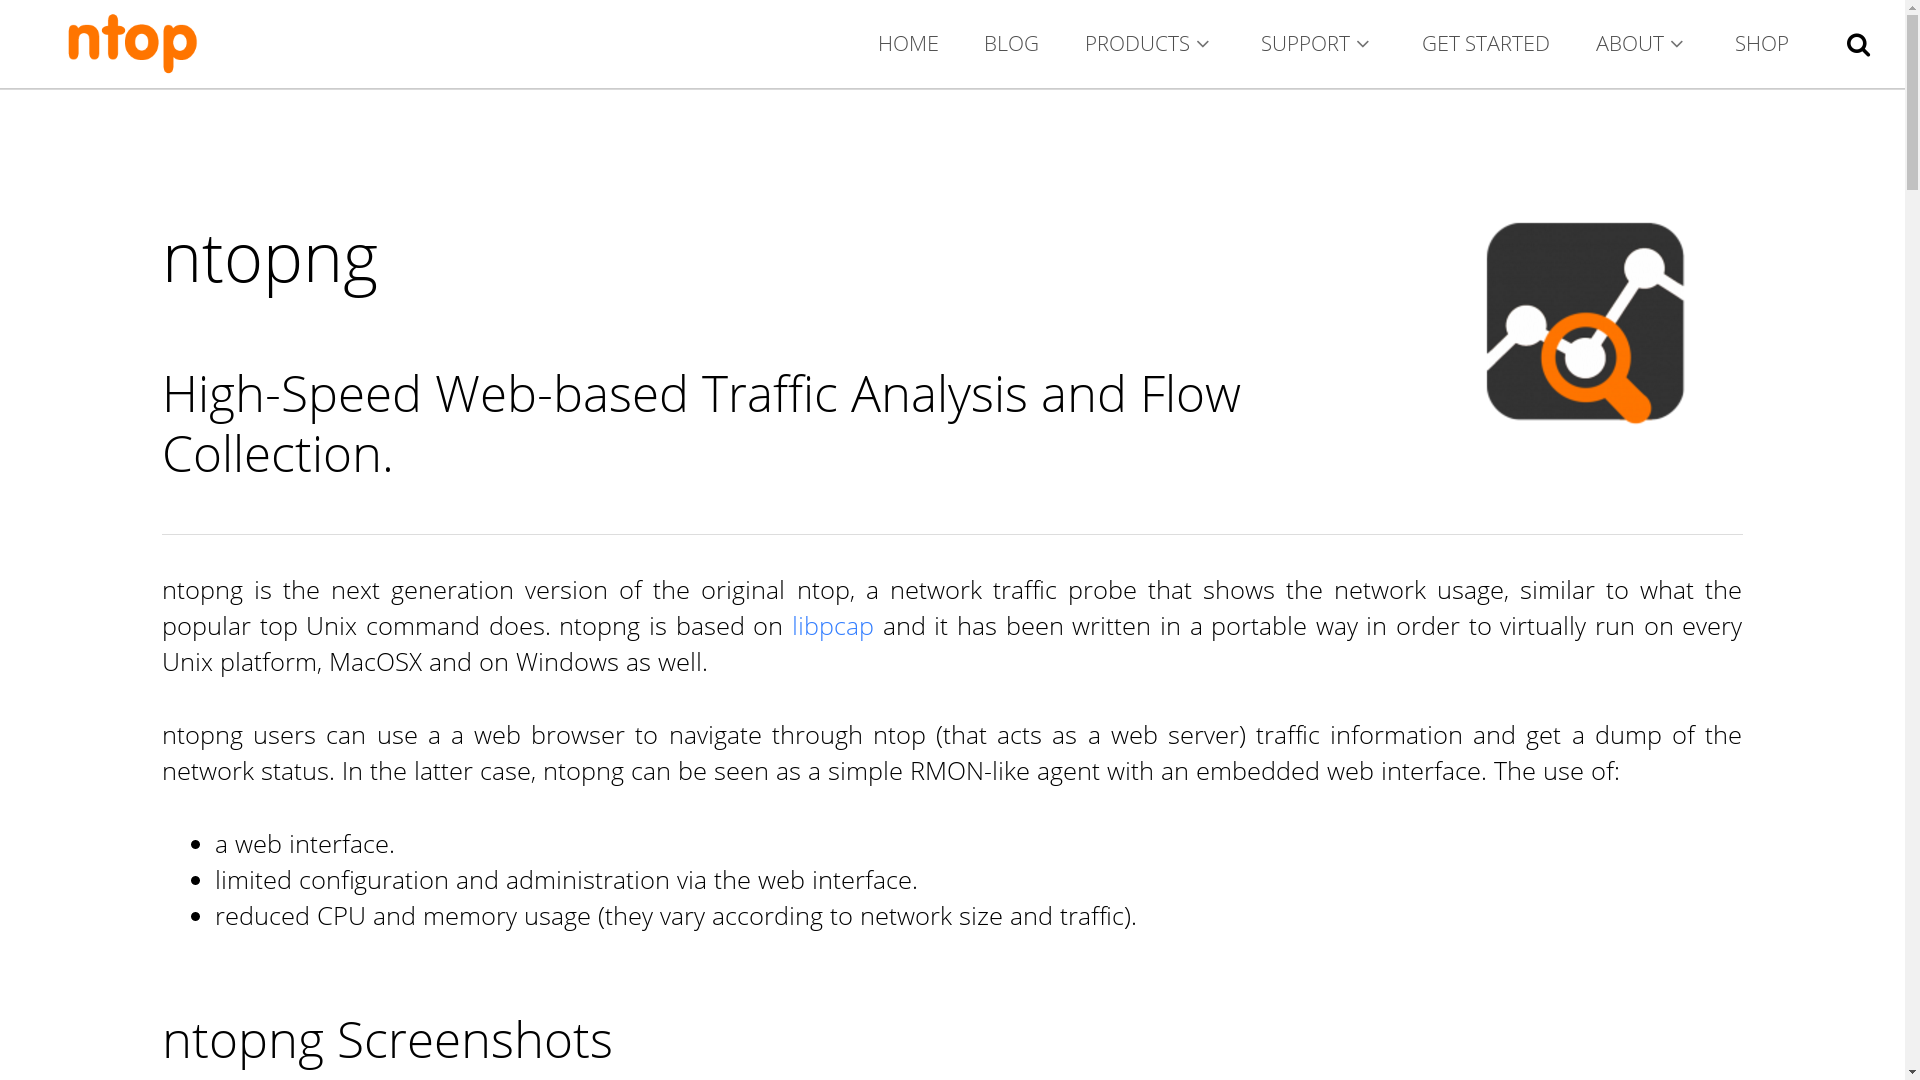
\includegraphics[keepaspectratio=true,height=0.50\textheight,width=0.75\textwidth,angle=0]{www-ntopng.png}
 \caption{ntopng Website}
 \label{fig:www-ntopng}
\end{center}
\end{figure}

\begin{itemize}
 \item Dashboard.
 \item Darkstat.
 \item ntopng (``Network Top Next Generation'' ?).
 \item S.M.A.R.T.
 \item System Temperatures.
 \item MRTG
 \item RRD
\end{itemize}


